	\section{Marco Teórico}
	
	Este capítulo establece los fundamentos teóricos y técnicos sobre los cuales se sustenta el presente trabajo terminal. Para comprender el diseño y la implementación del prototipo, es necesario abordar los conceptos clave de las distintas áreas de conocimiento involucradas.
	
	En primer lugar se aborda la LSM, analizando su estructura y relevancia en el contexto social. Posteriormente, se presentan los principios de la visión por computadora y los fundamentos del aprendizaje profundo, destacando el papel de las redes neuronales convolucionales (CNN) como una de las técnicas comúnmente empleadas en tareas de reconocimiento visual. También se consideran enfoques basados en la extracción de características mediante puntos clave de la mano (\textit{landmarks}).
	
	\subsection{LSM en México}
	
	La comunicación es un elemento fundamental para la vida social del ser humano, ya que permite el acceso a la información y la participación activa en distintos contextos. En la mayoría de los casos, la comunicación oral representa el medio principal de interacción sin embargo, cuando esta se ve limitada o impedida, las oportunidades de desarrollo educativo, profesional y social pueden verse significativamente restringidas \cite{sep2023lsm}.
	
	La discapacidad auditiva continúa siendo una de las condiciones menos tratadas dentro de los esfuerzos de inclusión social. A pesar de la existencia de marcos legales nacionales e internacionales, las personas sordas enfrentan diversas barreras, entre ellas físicas, comunicativas y actitudinales, que limitan su participación en ámbitos como la educación, el empleo y la vida comunitaria. Estas últimas, derivadas de prejuicios y estigmas sociales, se reflejan en la falta de disposición para establecer comunicación, así como en creencias erróneas sobre las capacidades de integración social y laboral de esta población. La LSM se reconoce como una herramienta esencial para garantizar la accesibilidad, la autonomía comunicativa y el ejercicio equitativo de derechos dentro de una sociedad inclusiva \cite{sanchez2022discapacidad}.
	
	No obstante, la falta de dominio de esta lengua por parte de la población oyente continúa representando un obstáculo significativo para la inclusión \cite{sep2023lsm}. Por eso es que el desarrollo de soluciones tecnológicas orientadas a reducir esta brecha adquiere una gran relevancia social.
	
	\subsubsection{Historia de la LSM}
	
	La Lengua de Señas Mexicana (LSM) es una lengua natural. Consiste en signos gestuales articulados con las manos, expresiones faciales, mirada intencional y movimiento corporal con función lingüística, que permiten expresar todo tipo de ideas, emociones, sentimientos y pensamientos a quienes la dominan. Posee sintaxis, gramática y léxico, siendo tan vasta y compleja como cualquier lengua oral \cite{ipn_lsm}.
	
	Desde 2003, la LSM fue declarada oficialmente como una lengua nacional, junto con las lenguas indígenas y el español, lo cual ha facilitado su uso en la educación de personas sordas. Anteriormente, la corriente educativa estaba enfocada en el oralismo, es decir, en enseñar a las personas sordas a leer los labios y utilizar la voz. De acuerdo con los Lineamientos Generales de Accesibilidad al Servicio de Televisión Radiodifundida, a partir de diciembre de 2018, los canales de televisión que se transmiten en el 50\% o más del territorio nacional deben contar con interpretación en LSM o subtitulaje oculto, lo que ha contribuido a dar mayor visibilidad a esta comunidad y su lengua \cite{cultura_lsm}.
	
	\subsubsection{Estructura lingüística de la LSM}
	
	La Lengua de Señas Mexicana (LSM) es un idioma completo con características lingüísticas propias que la diferencian estructuralmente del español. Su naturaleza es viso-gestual, lo que significa que la información se transmite y recibe a través de los canales visual y gestual en lugar del auditivo-vocal. A diferencia del español, que sigue una estructura gramatical predominantemente de Sujeto-Verbo-Objeto (SVO), la LSM puede emplear un orden distinto y utiliza el espacio tridimensional frente al signante para establecer relaciones gramaticales complejas \cite{ipn_lsm}.
	
	La construcción de cada seña se basa en un conjunto de parámetros formativos, equivalentes a los fonemas en las lenguas orales. Estos parámetros incluyen la configuración (forma de la mano), la ubicación (lugar del cuerpo donde se articula), el movimiento (la acción que se realiza), la orientación (la dirección de la palma) y los componentes no manuales (expresiones faciales y corporales que añaden información gramatical) \cite{sep2023lsm}.
	
	Dentro del léxico de la LSM, es fundamental distinguir entre el alfabeto dactilológico y las señas léxicas. El alfabeto dactilológico consiste en un conjunto de configuraciones manuales estáticas, donde cada una corresponde a una letra del alfabeto español. Su función principal es deletrear palabras que no cuentan con una seña específica, como nombres propios o términos técnicos. Por otro lado, las señas léxicas representa el vocabulario principal de la LSM, en donde un signo único representa un concepto completo \cite{cultura_lsm}.
	
	En las lenguas orales, la fonética distingue los diferentes fonemas mediante parámetros como el punto de articulación, el modo de articulación y la sonoridad. Por ejemplo, en español los fonemas /p/ y /b/ comparten características como ser oclusivos y bilabiales, diferenciándose en la sonoridad \cite{pressbooks_lsm}.
	
	En las lenguas de señas, como la LSM, se identifican cinco parámetros fundamentales que funcionan como unidades mínimas del gesto, de manera análoga a los fonemas en las lenguas orales. Estos parámetros son \cite{pressbooks_lsm}.:
	
	\begin{itemize}
		\item \textbf{Ubicación:} el punto o espacio corporal donde se efectúa la seña.
		
		\item \textbf{Movimiento:} la trayectoria u operación de la mano o manos que distingue un signo de otro.
		
		\item \textbf{Configuración de la mano:} la forma que adopta la mano dominante al realizar la seña.
		
		\item \textbf{Orientación:} la dirección en que la palma u otras partes de la mano se orientan durante el gesto.
		
		\item \textbf{Señales no manuales:} expresiones faciales, movimientos del cuerpo o del tronco que acompañan al gesto manual y son esenciales para el significado completo.
	\end{itemize}
	
	El parámetro de movimiento puede ser el único elemento diferenciador entre dos señas que comparten ubicación, configuración y orientación, lo que evidencia la complejidad estructural de la lengua gestual \cite{pressbooks_lsm}.
	
	\begin{figure}[H]
		\centering
		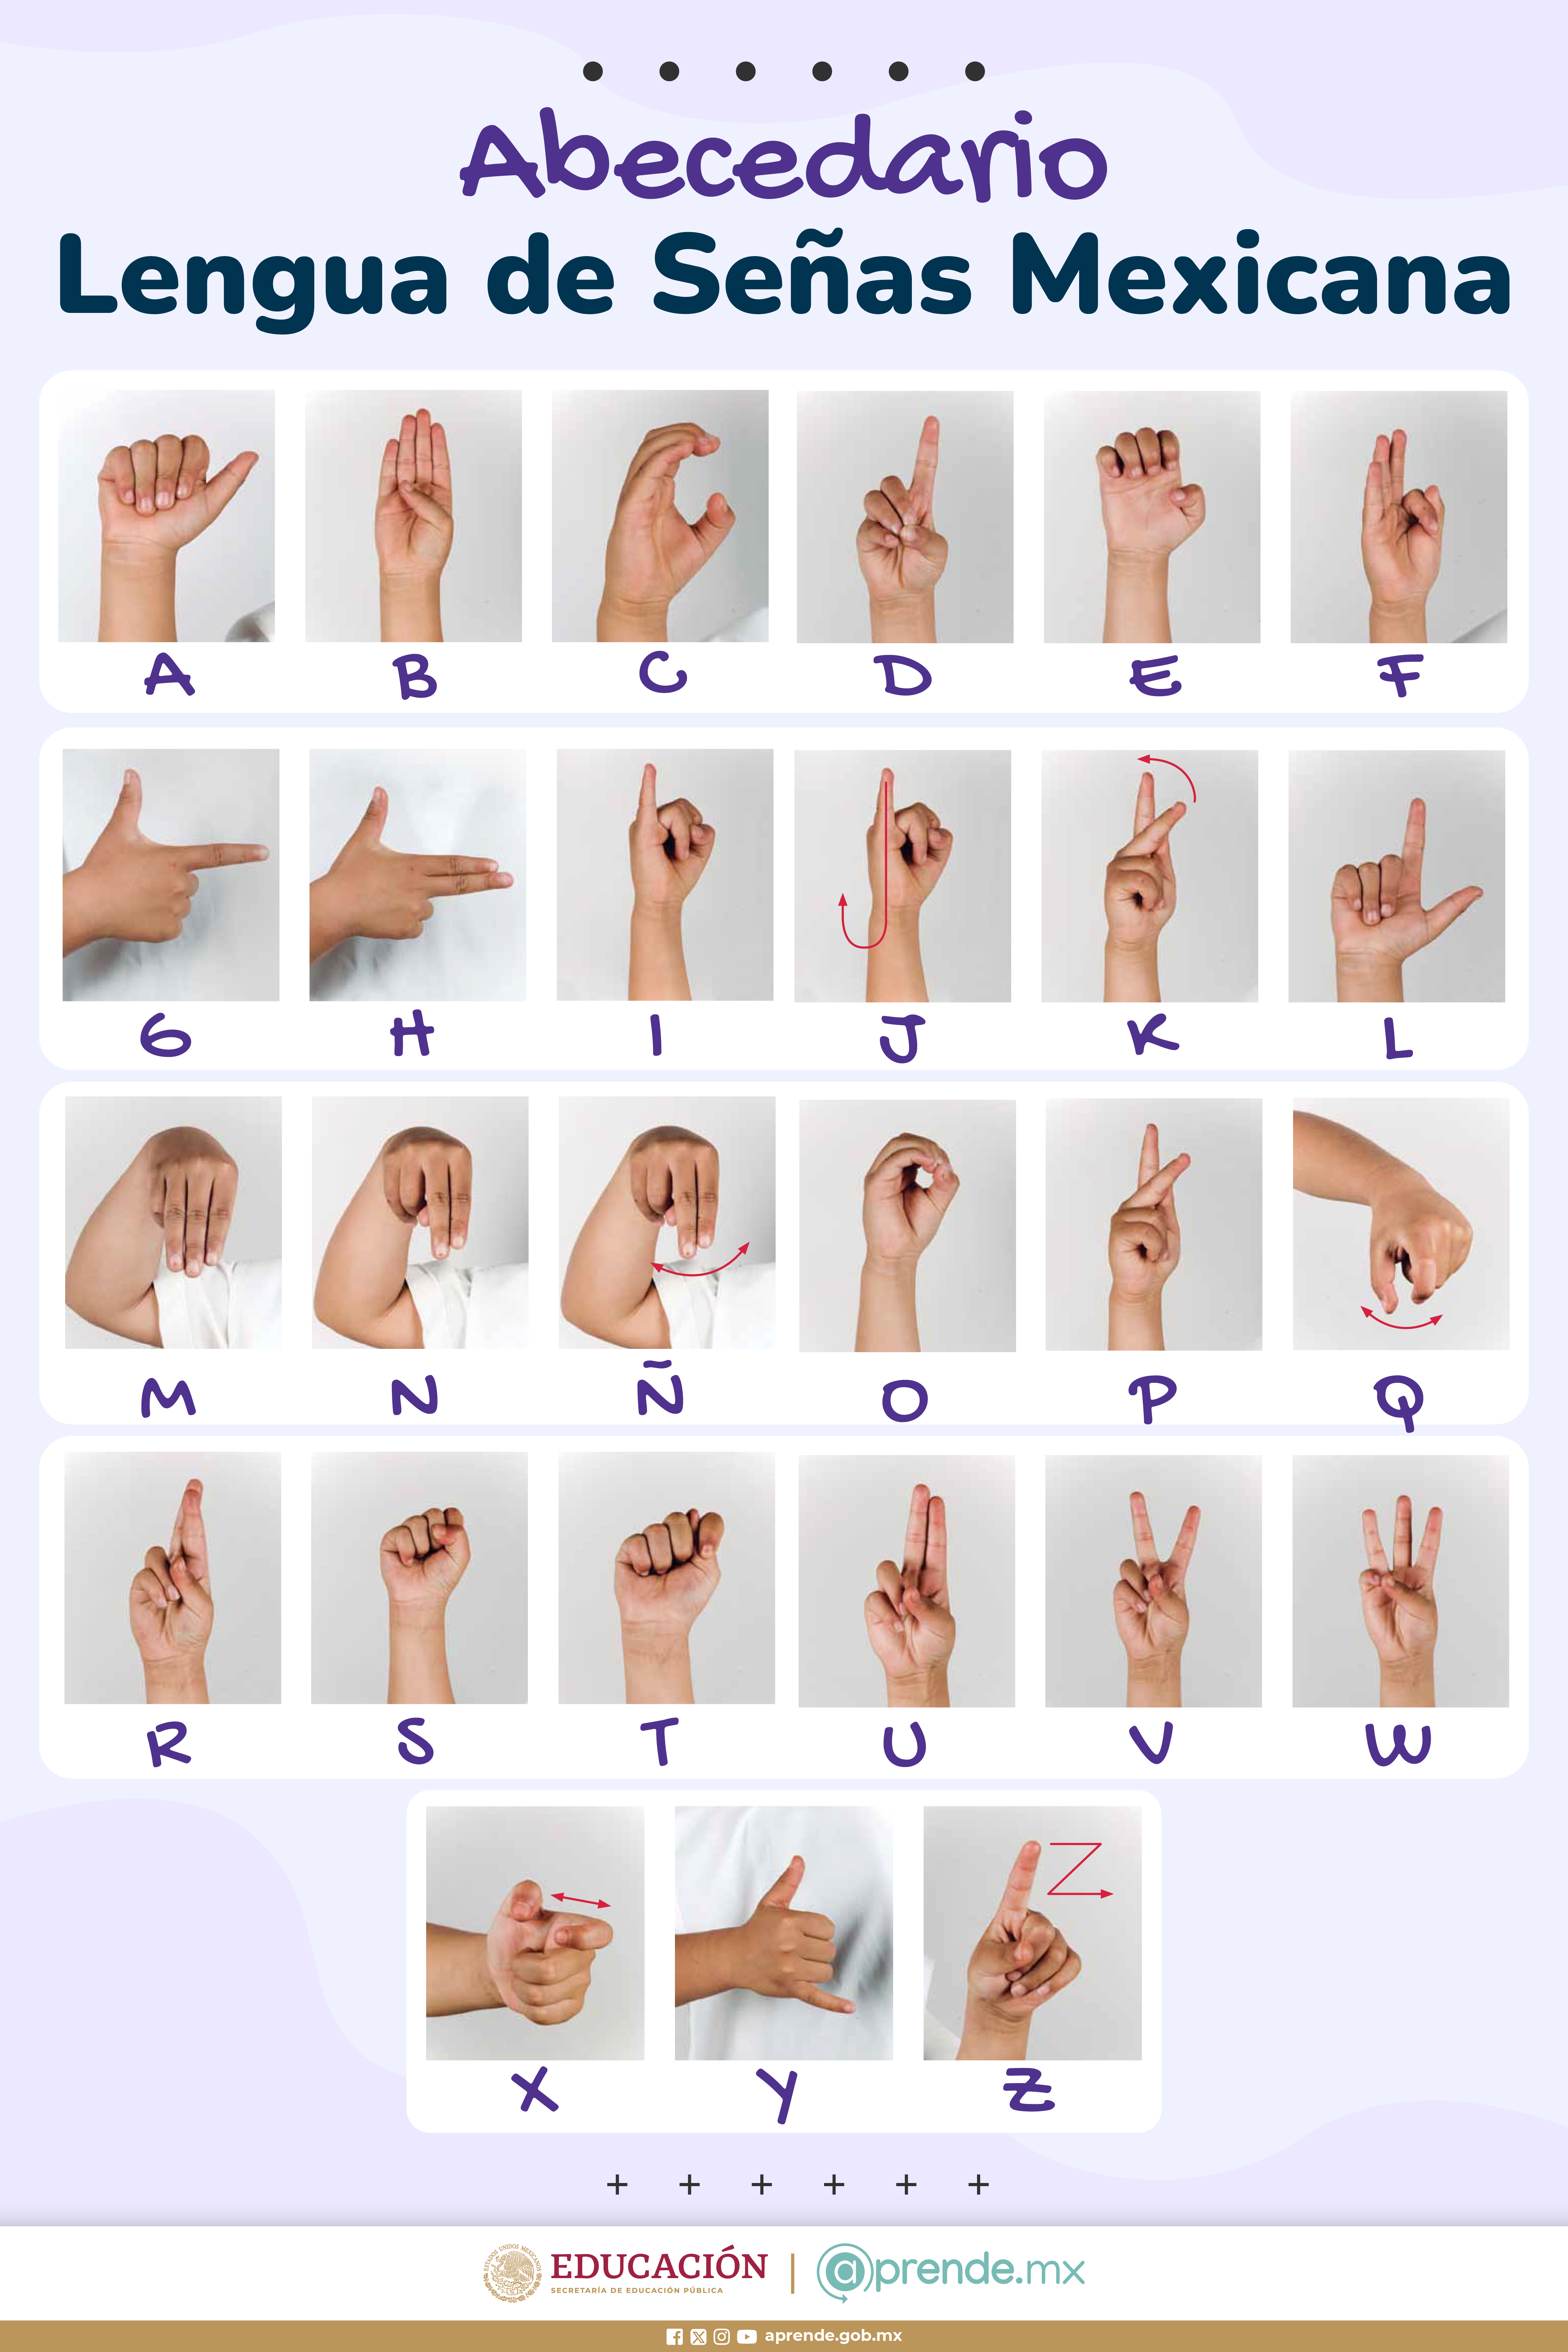
\includegraphics[width=0.7\textwidth]{images/Abecedario_LSM.jpg}
		\caption{Figura 1. Abecedario de la LSM\cite{sep_abecedario_lsm}.}
		\label{fig:mi_imagen}
	\end{figure}
	
	\subsubsection{Relevancia social: población y barreras de comunicación}
	
	En México, la comunidad sorda enfrenta importantes barreras de comunicación que limitan su desarrollo e inclusión social. La falta de datos censales precisos sobre el número de usuarios de la LSM dificulta la formulación de políticas públicas efectivas \cite{cultura_sorda_mexico}, aunque se estima que la población con discapacidad auditiva supera los 2.4 millones de personas \cite{cndh_lsm}.
	
	Esta comunidad enfrenta una exclusión sistemática derivada, en gran medida, de la escasez de intérpretes certificados en LSM, lo que genera una dependencia constante de familiares o terceros para la comunicación en ámbitos fundamentales como el hospitalario, legal y administrativo.
	
	Las barreras se manifiestan de manera crítica en el acceso a la justicia y a los servicios de salud. En el ámbito legal, las personas sordas pueden ser revictimizadas debido a la ausencia de intérpretes durante los procesos judiciales \cite{copred_sordos}. En el ámbito médico, la comunicación ineficaz puede derivar en diagnósticos incorrectos y en la vulneración del derecho al consentimiento informado \cite{castro2021barreras}.
	
	Esta situación no solo evidencia una brecha de comunicación, sino también una problemática estructural en el ejercicio de sus derechos humanos, ya que, a pesar de que la LSM es reconocida como lengua nacional, su uso no se encuentra plenamente garantizado en los servicios públicos \cite{cndh_lsm}.
	
	
	\subsubsection{Importancia en educación, inclusión y accesibilidad}
	
	La educación es uno de los ámbitos más afectados por las barreras de comunicación. Históricamente, el modelo educativo para personas sordas en México ha presentado diversas deficiencias, lo que ha derivado en que una parte significativa de esta población no concluya la educación básica. La falta de docentes bilingües (LSM–español) y de un modelo educativo verdaderamente inclusivo contribuye a perpetuar un ciclo de rezago y exclusión. En este sentido, el acceso a una educación de calidad desde la infancia resulta fundamental para garantizar el pleno desarrollo e inclusión social de las personas sordas \cite{copred_sordos}.
	
	Promover la inclusión y la accesibilidad no solo es un mandato legal, sino también un imperativo social. La Comisión Nacional de los Derechos Humanos (CNDH) señala que el Estado debe garantizar el derecho de las personas sordas a expresarse en su propia lengua \cite{cndh_lsm}. La accesibilidad va más allá de la presencia de intérpretes, ya que implica la creación de entornos en los que la LSM sea reconocida y utilizada en los distintos ámbitos de la vida, como los servicios gubernamentales, los medios de comunicación y los espacios culturales. Esto no solo favorece a la comunidad sorda, sino que también contribuye al fortalecimiento de una sociedad más inclusiva y respetuosa de la diversidad lingüística \cite{copred_sordos}.
	
	\subsection{Visión por Computadora}
	
	La interpretación automática de la LSM requiere transformar señales visuales en representaciones numéricas que puedan ser procesadas por un modelo de aprendizaje.
	
	La Visión por Computadora (VC), también conocida como visión artificial, es una rama de la Inteligencia Artificial inspirada en el sistema visual humano. Su objetivo principal es modelar y automatizar el proceso de reconocimiento visual, es decir, dotar a una computadora de la capacidad de distinguir entre diferentes objetos, imitando el proceso que realizan las personas para percibir y comprender una imagen \cite{cantero_vision}. Esta disciplina desarrolla técnicas matemáticas para recuperar la forma tridimensional y la apariencia de los objetos a partir de imágenes bidimensionales \cite{szeliski2022}.
	
	El desafío fundamental de la Visión por Computadora radica en que se trata de un problema inverso. A diferencia de la computación gráfica, que genera imágenes 2D a partir de modelos 3D (proceso directo), la VC busca describir y reconstruir propiedades del mundo tridimensional, como la forma, la iluminación y el color, a partir de proyecciones bidimensionales. Esta tarea es naturalmente compleja, ya que implica recuperar información desconocida a partir de datos limitados, lo que requiere el uso de modelos físicos, probabilísticos o de aprendizaje automático para aproximar una solución \cite{szeliski2022}.
	
	A pesar de esta complejidad, la Visión por Computadora se ha consolidado como una tecnología clave en múltiples aplicaciones del mundo real, tanto en el ámbito industrial como en el de consumo. Entre sus aplicaciones destacan el reconocimiento óptico de caracteres (OCR), la inspección de piezas en control de calidad, el análisis de imágenes médicas, los vehículos autónomos, la generación de imágenes panorámicas y la detección de rostros, entre otras \cite{szeliski2022}. De manera general, un sistema de visión artificial sigue una serie de etapas bien definidas: adquisición de la imagen, preprocesamiento, segmentación de los objetos de interés y, finalmente, reconocimiento e interpretación de la escena \cite{cantero_vision}.
	
	\subsubsection{La imagen digital y modelos de color}
	
	Para comprender cómo la visión por computadora interpreta las imágenes, el primer paso es analizar su materia prima fundamental: la imagen digital. A diferencia de la percepción humana, una computadora no “ve” una escena, sino que la procesa como una estructura de datos numéricos. Por ello, es necesario definir los elementos que componen esta estructura, desde su unidad más básica, el píxel, hasta la forma en que se representa el color \cite{szeliski2022}.
	
	Existen diversas formas de adquirir imágenes; sin embargo, el objetivo en todos los casos es el mismo: generar imágenes digitales a partir de los datos captados por sensores. La salida de la mayoría de estos sensores es una señal continua de voltaje, cuya amplitud y comportamiento espacial están relacionados con el fenómeno físico detectado. Para convertir estos datos continuos en una imagen digital, es necesario aplicar dos procesos fundamentales: muestreo y cuantificación \cite{szeliski2022, gonzalez2018}.
	
	El muestreo consiste en discretizar las coordenadas espaciales de la imagen mediante su división en una cuadrícula, mientras que la cuantificación implica asignar un valor numérico discreto a cada punto de dicha cuadrícula, representando su nivel de intensidad \cite{gonzalez2018}.
	
	El resultado de estos procesos es el píxel (del inglés \textit{picture element}), la unidad más pequeña de una imagen digital, la cual posee una posición y un valor de intensidad. De esta manera, la computadora representa una imagen como una matriz o arreglo bidimensional de valores numéricos, como se ilustra en la Figura \ref{fig:imagen_digital}.
	
	\begin{figure}[H]
		\centering
		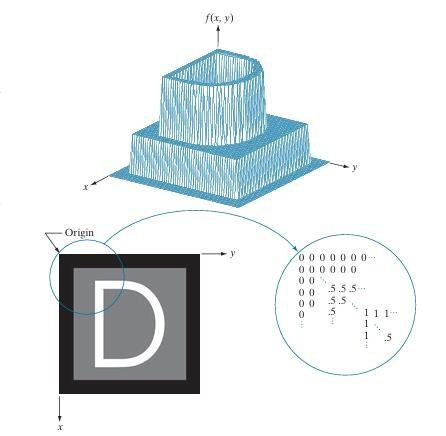
\includegraphics[width=0.4\textwidth]{images/fig2.jpg}
		\caption{Tres formas de representar una imagen: (a) como superficie, (b) como se ve en pantalla, y (c) como una matriz de píxeles \cite{szeliski2022}.}
		\label{fig:imagen_digital}
	\end{figure}
	 
	 
	 Esta matriz se rige por un sistema de coordenadas en el cual el origen (0,0) se ubica comúnmente en la esquina superior izquierda. En este sistema, el eje x avanza hacia la derecha (columnas), mientras que el eje y avanza hacia abajo (filas) \cite{gonzalez2018}.
	 
	 
	\begin{figure}[H]
		\centering
		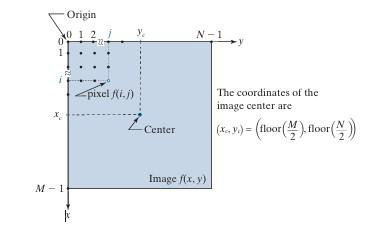
\includegraphics[width=0.5\textwidth]{images/fig3.jpg}
		\caption{Representación de un sistema de coordenadas de una imagen digital, donde un píxel se denota como f(i, j)  \cite{gonzalez2018}.}
		\label{fig:sistema_cordenadas}
	\end{figure}
	
	Matemáticamente, una imagen digital de $M$ filas y $N$ columnas puede representarse como una función $f(x,y)$ o como una matriz $A$, donde cada elemento corresponde al valor de intensidad de un píxel \cite{gonzalez2018}. A continuación, se muestra su representación:
	
	\begin{equation*}
		\small
		f(x,y)=
		\left[
		\begin{array}{cccc}
			f(0,0) & f(0,1) & \cdots & f(0,N-1) \\
			f(1,0) & f(1,1) & \cdots & f(1,N-1) \\
			\vdots & \vdots & \ddots & \vdots \\
			f(M-1,0) & f(M-1,1) & \cdots & f(M-1,N-1)
		\end{array}
		\right]
	\end{equation*}
	
	De manera equivalente, puede expresarse como una matriz:
	
	\begin{equation*}
		\small
		A=
		\left[
		\begin{array}{cccc}
			a_{0,0} & a_{0,1} & \cdots & a_{0,N-1} \\
			a_{1,0} & a_{1,1} & \cdots & a_{1,N-1} \\
			\vdots & \vdots & \ddots & \vdots \\
			a_{M-1,0} & a_{M-1,1} & \cdots & a_{M-1,N-1}
		\end{array}
		\right]
	\end{equation*}
	
	donde $f(x,y)$ o $a_{i,j}$ representan el valor de intensidad del píxel en la posición correspondiente dentro de la imagen.
	
	Una vez que la imagen ha sido muestreada y cuantizada, es necesario definir cómo se representará numéricamente el color de cada píxel. El modelo más común es el RGB (Rojo, Verde, Azul), un modelo de color aditivo que simula la emisión de luz mediante la combinación de estos tres colores primarios para generar un amplio espectro cromático. En la práctica, una imagen RGB se compone de tres matrices o canales independientes, cada uno representando la intensidad de uno de los colores primarios \cite{xian2025}.
	
	Si bien el modelo RGB es fundamental para la captura y visualización de imágenes a color, muchas tareas de visión por computadora se centran en las características estructurales de los objetos, como sus bordes y formas, en lugar de su color. En estos casos, la información de los tres canales puede simplificarse en una única representación basada en la intensidad luminosa.
	
	Una imagen en escala de grises se representa mediante una sola matriz de datos, en la cual cada elemento corresponde al nivel de luminancia (brillo) del píxel. Esta representación elimina la información de crominancia (matiz y saturación), conservando únicamente la intensidad de la luz.
	
	En el modelo RGB, la luminancia se encuentra combinada con la crominancia. Para aislar el componente de luminancia (denotado como $Y$), el cual se aproxima a la percepción humana del brillo, se utiliza una conversión estándar a partir de los canales RGB, definida como:
	
	\begin{equation*}
		Y = 0.299R + 0.587G + 0.114B
	\end{equation*}
	
	Esta separación de la imagen en sus componentes de luminancia y crominancia es un factor de diseño relevante en el Aprendizaje Profundo. Investigaciones como las de Xian \cite{xian2025} han demostrado que la selección del espacio de color puede afectar significativamente la precisión de la clasificación en Redes Neuronales Convolucionales (CNN). Al disponer del brillo en un canal independiente del color, como en los espacios LAB o YCbCr, los modelos pueden ser más robustos ante variaciones en las condiciones de iluminación, ya que diferentes espacios de color enfatizan distintos aspectos de la información visual \cite{ballester2022}.
	
	Por esta razón, en muchas tareas de Visión por Computadora enfocadas en el reconocimiento de formas como en el presente proyecto, resulta una práctica común y justificada convertir las imágenes a escala de grises. Este proceso reduce la complejidad computacional (de tres canales a uno) y, al aislar el componente de luminancia, permite que el modelo se enfoque en las características estructurales del objeto, tales como bordes, contornos y formas\cite{ballester2022, xian2025}.
	
	\subsubsection{Técnicas de preprocesamiento de imágenes}
	
	Cuando obtiene la representación digital de una imagen, esta rara vez puede ser utilizada directamente para su análisis. Las imágenes capturadas suelen ser de naturaleza “cruda” y están sujetas a una alta variabilidad, incluyendo diferencias de tamaño, condiciones de iluminación no controladas y la presencia de ruido digital introducido por el propio sensor de la cámara \cite{cantero_vision, gonzalez2018}.
	
	Es por eso que el preprocesamiento de imágenes se considera una etapa fundamental en la mayoría de los sistemas de Visión por Computadora \cite{szeliski2022, gonzalez2018}. Su objetivo es mejorar la calidad de la imagen, limpiar y estandarizar los datos visuales, mediante la aplicación de una serie de operaciones que permiten minimizar variaciones irrelevantes y resaltar las características importantes. Esta preparación asegura que las etapas posteriores de análisis, como la extracción de características o la clasificación mediante modelos de aprendizaje automático, reciban datos consistentes y de alta calidad, lo cual resulta indispensable para obtener un desempeño preciso y robusto \cite{cantero_vision, szeliski2022, gonzalez2018}.
	
	El redimensionamiento (\textit{resizing}) es una de las operaciones de preprocesamiento más comunes y fundamentales en los sistemas de clasificación de imágenes. Su objetivo principal es ajustar las dimensiones espaciales de una imagen para que todas las entradas tengan un tamaño fijo y estandarizado, por ejemplo, $224 \times 224$ píxeles.
	
	La necesidad de este paso se fundamenta en tres razones técnicas principales:
	
	\begin{enumerate}
		\item \textbf{Procesamiento por lotes (mini-batch):} Los métodos de entrenamiento basados en descenso de gradiente requieren que todas las imágenes dentro de un mismo lote tengan la misma resolución espacial, lo que permite su procesamiento eficiente en paralelo \cite{talebi2021}.
		
		\item \textbf{Limitaciones de memoria:} El hardware utilizado, como las unidades de procesamiento gráfico (GPU), cuenta con memoria limitada, lo que restringe el uso de imágenes de alta resolución durante el entrenamiento y la inferencia \cite{talebi2021}.
		
		\item \textbf{Eficiencia computacional:} El uso de imágenes de gran tamaño incrementa significativamente el costo computacional, afectando tanto el tiempo de entrenamiento como la velocidad de inferencia del modelo \cite{talebi2021}.
	\end{enumerate}
	
	Históricamente, los métodos más comunes para realizar el redimensionamiento han sido algoritmos de interpolación, como el bilineal o el bicúbico. Sin embargo, la literatura reciente ha señalado que estos métodos, aunque eficientes, fueron diseñados antes del auge del Aprendizaje Profundo y no están optimizados para tareas de visión por computadora orientadas a modelos de aprendizaje automático.
	
	Diversos estudios han demostrado que la elección del método de redimensionamiento puede influir de manera significativa en el rendimiento final de la tarea. En este sentido, las investigaciones actuales sugieren que los algoritmos más adecuados para tareas de visión por computadora no necesariamente coinciden con aquellos diseñados para producir imágenes visualmente agradables para el ojo humano \cite{talebi2021}.
	
	
	\begin{figure}[H]
		\centering
		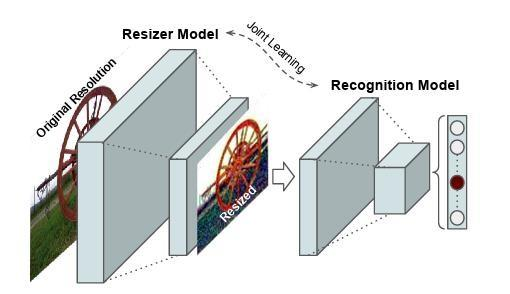
\includegraphics[width=0.4\textwidth]{images/fig4.jpg}
		\caption{Modelos de Redimensionamiento y Reconocimiento\cite{talebi2021}.}
		\label{fig:Redimensionamiento}
	\end{figure}
	
	Después de estandarizar el tamaño de las imágenes mediante el redimensionamiento, el siguiente paso en el preprocesamiento consiste en mejorar la calidad del contenido visual. Las imágenes capturadas por sensores digitales, específicamente en condiciones de iluminación no ideales, suelen contener ruido, el cual se manifiesta como variaciones aleatorias en la intensidad o el color de los píxeles \cite{gonzalez2018}. 
	
	La importancia de esta etapa radica en que la presencia de ruido puede afectar significativamente la exactitud de los procesos de análisis basados en imágenes, convirtiendo su reducción en uno de los principales desafíos del procesamiento de imágenes. El ruido altera características fundamentales como los bordes, la nitidez y el contraste \cite{xian2025}, que son precisamente los atributos utilizados por los modelos de aprendizaje para distinguir entre diferentes objetos, formas o patrones \cite{betancourt2003}. 
	
	Por lo tanto, la aplicación de técnicas de reducción de ruido (\textit{denoising}) se considera una etapa fundamental para mejorar la calidad de la imagen y asegurar que los modelos aprendan a partir de características estructurales relevantes, evitando la influencia de artefactos aleatorios.
	
	Existen distintos tipos de ruido que pueden contaminar una imagen. Entre los más comunes se encuentran:
	
	\begin{itemize}
		\item \textbf{Ruido Gaussiano:} Se manifiesta como variaciones continuas en la intensidad de los píxeles a lo largo de toda la imagen. Generalmente es causado por los componentes electrónicos del sensor de la cámara \cite{mateu2017}.
		
		\item \textbf{Ruido impulsivo (sal y pimienta):} Se caracteriza por la aparición de píxeles aislados con valores extremos, ya sea muy altos (blancos) o muy bajos (negros). Este tipo de ruido suele generarse en procesos de adquisición o cuantización \cite{mateu2017}.
	\end{itemize}
	
	Para atenuar estos efectos, se emplean filtros espaciales, que son algoritmos de suavizado que operan sobre un píxel y su vecindario. Un enfoque común es el uso de filtros pasa-bajas, como el filtro de media o el filtro gaussiano. El filtro de media reemplaza el valor de cada píxel por el promedio de sus vecinos, logrando un efecto de suavizado general.
	
	Sin embargo, aunque estos filtros son efectivos para reducir el ruido, también pueden difuminar los bordes y disminuir la nitidez de la imagen. Por ello, la selección del método de filtrado implica un compromiso entre la reducción del ruido y la preservación de las características relevantes, como los contornos, que son esenciales para tareas de reconocimiento \cite{mateu2017}.
	
	\begin{figure}[H]
		\centering
		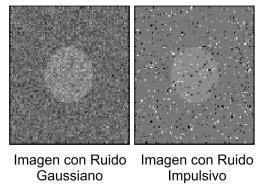
\includegraphics[width=0.4\textwidth]{images/fig5.jpg}
		\caption{Ruido Gaussiano e impulsivo en una imagen \cite{betancourt2003}.}
		\label{fig:ruido}
	\end{figure}
	
	
	La última etapa fundamental del preprocesamiento es la normalización de la imagen. Esta operación no modifica la apariencia visual de la imagen, sino que estandariza los valores numéricos de sus píxeles \cite{albert2023}. Cuando se trabaja con conjuntos de datos provenientes de múltiples fuentes, como imágenes capturadas por diferentes dispositivos o en condiciones de iluminación variables, los datos presentan una alta variabilidad. Para reducir estos efectos, se aplican técnicas de normalización como parte del preprocesamiento.
	
	La importancia de la normalización radica en su impacto directo sobre la capacidad de generalización de los modelos de aprendizaje. Un modelo entrenado con datos no normalizados puede presentar dificultades para adaptarse a nuevas imágenes con distribuciones de intensidad distintas a las observadas durante el entrenamiento. Al estandarizar los datos, se favorece el aprendizaje de características estructurales del objeto de interés, en lugar de sesgos derivados de variaciones de iluminación \cite{albert2023}.
	
	El objetivo de la normalización es transformar los valores de los píxeles, originalmente en un rango como $[0,255]$, a una escala común y consistente. Este proceso contribuye a mejorar la eficiencia, estabilidad y capacidad de generalización de los modelos \cite{goodfellow2016}. En particular, la normalización acelera la convergencia en el proceso del entrenamiento, ya que el aprendizaje es más eficiente cuando las características de entrada presentan valores centrados alrededor de cero \cite{lecun1998}.
	
	Ademas ayuda a estabilizar el proceso de aprendizaje al prevenir problemas como la explosión o el desvanecimiento de gradientes, permitiendo actualizaciones más controladas de los parámetros del modelo \cite{goodfellow2016}. La estandarización de los datos es el último paso y ayuda a reducir la complejidad del problema en cuestión, favoreciendo que el modelo aprenda patrones relevantes en lugar de adaptarse a variaciones específicas del conjunto de entrenamiento \cite{ioffe2015, bishop2006}.
	
	A continuación, se describen dos de las técnicas de normalización más utilizadas:
	
	La estandarización (\textit{Z-score normalization}) es una de las técnicas más robustas y comúnmente empleadas en aplicaciones de visión por computadora \cite{bishop2006}. Esta transforma la distribución de los valores de intensidad de los píxeles para que tengan una media ($\mu$) de 0 y una desviación estándar ($\sigma$) de 1. La transformación para cada píxel $x$ se define como:
	
	\begin{equation}
		x' = \frac{x - \mu}{\sigma}
	\end{equation}
	
	donde $x'$ es el valor normalizado, $x$ es el valor original del píxel, y $\mu$ y $\sigma$ corresponden a la media y desviación estándar calculadas sobre el conjunto de datos de entrenamiento. Esta técnica fue utilizada en arquitecturas influyentes como AlexNet, donde se realizaba una sustracción de la media para centrar los datos \cite{krizhevsky2012}.
	
	Una técnica alternativa es el escalado Mín–Máx, que ajusta los valores de los píxeles a un rango predefinido, comúnmente $[0,1]$ \cite{bishop2006}. Esta transformación lineal se expresa como:
	
	\begin{equation}
		x' = \frac{x - \min(x)}{\max(x) - \min(x)}
	\end{equation}
	
	donde $\min(x)$ y $\max(x)$ representan los valores mínimo y máximo de intensidad en la imagen (usualmente 0 y 255, respectivamente). Aunque este método es computacionalmente simple, la estandarización suele ser preferida por su mayor robustez frente a variaciones en las condiciones de iluminación \cite{goodfellow2016}.
	
	
	\subsubsection{Segmentación de objetos}
	
	Después de que la imagen ha sido acondicionada mediante técnicas de preprocesamiento, el siguiente desafío consiste en identificar qué regiones contienen la información relevante. Una imagen capturada por una cámara no solo incluye el objeto de interés, sino también un contexto visual —como paredes, muebles u otros elementos del entorno— que no contribuyen al análisis.
	
	Se introduce el concepto de segmentación de objetos. El objetivo de esta etapa es delimitar y aislar los píxeles que corresponden al objeto de interés (en este caso, la mano) del resto de la escena. Este proceso permite enfocar el análisis posterior únicamente en las características relevantes de la seña.
	
	Para abordar este problema, se emplea la segmentación de imágenes, una técnica de visión por computadora que divide una imagen digital en grupos discretos de píxeles, denominados segmentos, con el fin de facilitar la detección de objetos y otras tareas de análisis \cite{bishop2006, ibm_segmentation}. Al descomponer una imagen en regiones más simples y estructuradas, la segmentación permite un procesamiento más eficiente y preciso. En la interacción humano-computadora, su función principal es identificar y aislar los objetos de interés del fondo \cite{ibm_segmentation}.
	
	El campo de la segmentación de imágenes se divide en diversas tareas, cada una con un propósito específico. La más relevante para este trabajo es la segmentación semántica, cuyo objetivo es asignar una etiqueta de clase a cada píxel de la imagen \cite{szeliski2022, hao2020}. A diferencia de la segmentación por instancia, que distingue entre múltiples objetos de la misma categoría, la segmentación semántica agrupa todos los píxeles pertenecientes a una misma clase.
	
	De esta forma, esta técnica permite clasificar la imagen a nivel de píxel, facilitando la identificación del conjunto completo de píxeles que conforman el objeto de interés y su separación del fondo \cite{ibm_segmentation}.
	
	La Figura~\ref{fig:vision} ilustra las diferencias entre las principales tareas de la visión por computadora. A partir de una imagen de entrada, la segmentación semántica asigna una etiqueta a cada píxel, dividiendo la imagen en regiones mutuamente excluyentes que representan áreas significativas dentro de la escena \cite{hao2020}.
	
	\begin{figure}[H]
		\centering
		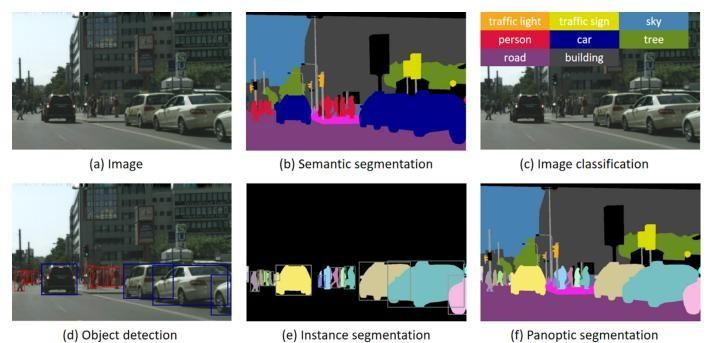
\includegraphics[width=0.8\textwidth]{images/fig6.jpg}
		\caption{Comparación de diferentes tareas de visión por computadora  \cite{hao2020}.}
		\label{fig:vision}
	\end{figure}
	
	Esta tarea se distingue claramente de otras tareas fundamentales de la visión por computadora:
	
	\begin{itemize}
		\item \textbf{Clasificación de imágenes (Fig.~6c):} Asigna una o más etiquetas a la imagen completa. Permite identificar qué objetos están presentes en la escena (por ejemplo, \textit{person}, \textit{car}, \textit{road}), pero no proporciona información sobre su ubicación \cite{hao2020}.
		
		\item \textbf{Detección de objetos (Fig.~6d):} Extiende la clasificación al incluir información espacial. Además de identificar los objetos presentes, determina su localización mediante regiones delimitadas, generalmente representadas por rectángulos o \textit{bounding boxes} \cite{hao2020}.
		
		\item \textbf{Segmentación semántica (Fig.~6b):} Representa un nivel de detalle mayor, ya que asigna una etiqueta de clase a cada píxel de la imagen. En lugar de delimitar los objetos mediante regiones aproximadas, define con precisión sus contornos, separándolos del fondo \cite{hao2020}.
	\end{itemize}
	
	
	La dificultad de la segmentación semántica radica en varios factores clave. En primer lugar, debe cerrar la brecha entre las características visuales de bajo nivel (píxeles) y la semántica de alto nivel (el concepto abstracto de un objeto) \cite{hao2020}. En segundo lugar, debe enfrentarse a fondos complejos o caóticos, donde la distinción visual entre el objeto y el entorno puede ser mínima, o donde coexisten múltiples objetos con características similares. Las variaciones inherentes a la forma del objeto, las condiciones de iluminación y la pose añaden niveles adicionales de complejidad \cite{barik2010}.
	
	A pesar de estos desafíos, la segmentación semántica es fundamental en numerosas aplicaciones prácticas, como la conducción autónoma, la detección de peatones y el diagnóstico médico asistido por computadora \cite{barik2010}. Al proporcionar una representación detallada a nivel de píxel, permite a los sistemas inteligentes comprender la escena con mayor precisión y tomar decisiones informadas \cite{hao2020}.
	
	Históricamente, la segmentación de imágenes se abordó mediante métodos clásicos, como ecuaciones diferenciales parciales y algoritmos basados en aprendizaje automático tradicional, como los bosques aleatorios \cite{hao2020}. Sin embargo, el auge de las redes neuronales profundas ha impulsado significativamente el desarrollo de esta área, logrando mejoras sustanciales en términos de precisión y robustez \cite{barik2010}.
	
	Para lograr la partición de la imagen, se han desarrollado diversas técnicas. De manera general, los enfoques clásicos se basan en propiedades de bajo nivel de los píxeles y en su relación espacial. Entre las familias más representativas se encuentran:
	
	\begin{itemize}
		\item \textbf{Umbralización (\textit{thresholding}):} Consiste en seleccionar uno o varios umbrales de intensidad para separar los píxeles en distintas clases, por ejemplo, objeto y fondo \cite{jain1989}. 
		
		Variantes como la umbralización adaptativa permiten calcular el umbral de forma local, lo que mejora su desempeño en condiciones de iluminación no uniformes \cite{shapiro2001}. De acuerdo con la documentación de OpenCV \cite{opencv_docs}, el método \texttt{cv2.adaptiveThreshold()} implementa un esquema basado en una media ponderada mediante una función gaussiana en una ventana local, permitiendo una segmentación más robusta ante variaciones de iluminación.
	\end{itemize}
	
	\begin{figure}[H]
		\centering
		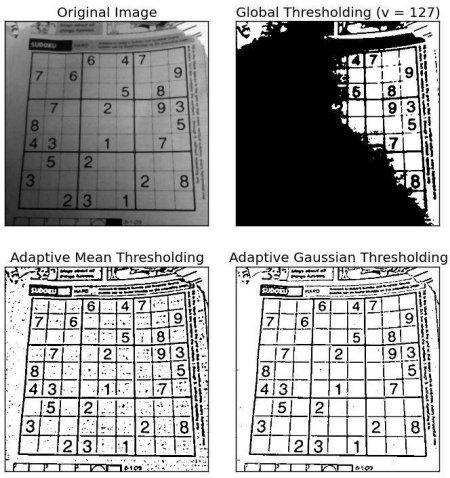
\includegraphics[width=0.4\textwidth]{images/fig7.jpg}
		\caption{Comparación entre diferentes métodos de umbralización implementados en OpenCV: global, adaptativa por media y adaptativa gaussiana  \cite{opencv_docs}.}
		\label{fig:ruido}
	\end{figure}
	
	\textbf{Detección de bordes:} consiste en identificar discontinuidades abruptas en la intensidad de la imagen, bajo la suposición de que dichas variaciones corresponden a los límites entre objetos. Este proceso se basa en el análisis del gradiente de intensidad, el cual permite resaltar cambios significativos en los niveles de brillo. Para ello, se emplean operadores como Sobel y Canny, ampliamente utilizados en el procesamiento de imágenes para la detección de bordes \cite{jain1989,shapiro2001}.
	
	\begin{figure}[H]
		\centering
		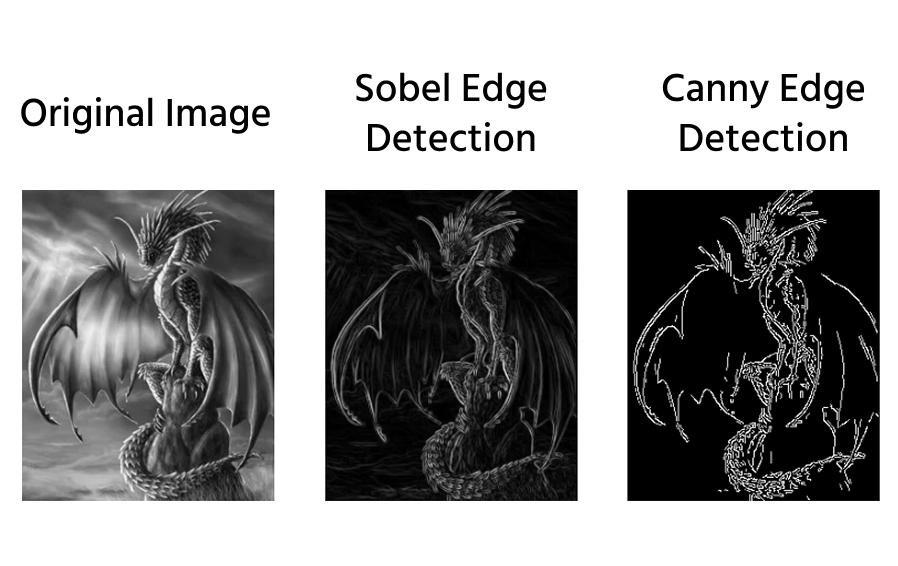
\includegraphics[width=0.6\textwidth]{images/fig8.jpg}
		\caption{Comparativa de deteccion de bordes  \cite{codefinity_vc}.}
		\label{fig:sobel}
	\end{figure}
	
	\textbf{Crecimiento de regiones:} es una técnica de segmentación que inicia a partir de uno o varios píxeles denominados “semillas” y expande la región agregando píxeles vecinos que cumplen un criterio de homogeneidad, como la similitud de intensidad o color. El proceso continúa de manera iterativa hasta que no es posible incorporar nuevos píxeles que satisfagan dicho criterio, permitiendo así delimitar regiones coherentes dentro de la imagen \cite{shapiro2001}.
	
	\textbf{Umbralización de Otsu:} es una técnica avanzada de segmentación utilizada cuando la imagen presenta una distribución bimodal en los valores de intensidad. A diferencia de los métodos de umbralización simple o adaptativa, el método de Otsu determina automáticamente el umbral óptimo mediante el análisis del histograma de la imagen, maximizando la varianza entre clases. Esto es útil cuando no se conoce previamente el valor adecuado del umbral \cite{geeksforgeeks_otsu}.
	
	\begin{figure}[H]
		\centering
		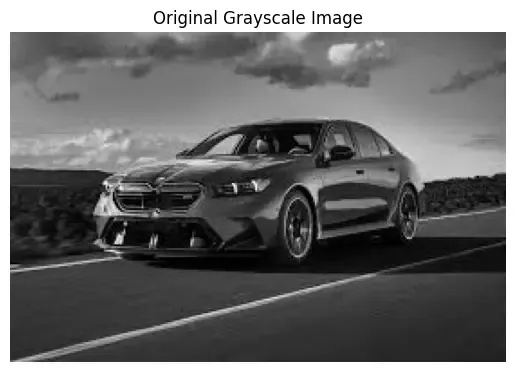
\includegraphics[width=0.6\textwidth]{images/fig9.png}
		\caption{Imagen original en escala de grises \cite{geeksforgeeks_otsu}.}
		\label{fig:sobel}
	\end{figure}
	
	\begin{figure}[H]
		\centering
		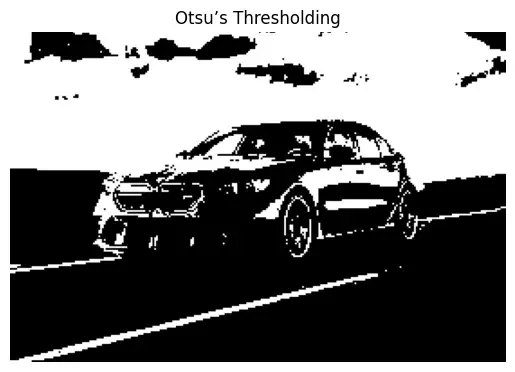
\includegraphics[width=0.6\textwidth]{images/fig10.png}
		\caption{Aplicando umbralización de Otsu \cite{geeksforgeeks_otsu}.}
		\label{fig:sobel}
	\end{figure}
	
	
	Si bien los métodos clásicos de segmentación son eficientes, el uso de CNN ha revolucionado la segmentación semántica, permitiendo alcanzar niveles de precisión significativamente superiores en comparación con enfoques tradicionales \cite{barik2010}.
	
	El enfoque moderno predominante se basa en arquitecturas de tipo codificador-decodificador (Encoder-Decoder), las cuales permiten capturar tanto el contexto semántico como la localización espacial de los objetos. En este esquema, el codificador se encarga de extraer características de alto nivel mediante la reducción progresiva de la resolución de la imagen, mientras que el decodificador reconstruye la información espacial mediante técnicas de \textit{upsampling}, generando finalmente una máscara de segmentación \cite{garcia2017review}. 
	
	Diversas arquitecturas han implementado y perfeccionado este enfoque. Modelos como Fully Convolutional Networks (FCN), SegNet y U-Net han demostrado un alto desempeño en tareas de segmentación, incorporando mecanismos como las conexiones de salto (\textit{skip connections}), las cuales permiten preservar información de diferentes niveles de resolución, mejorando la precisión en la delimitación de los bordes \cite{ronneberger2015unet}.
	
	
	\begin{figure}[H]
		\centering
		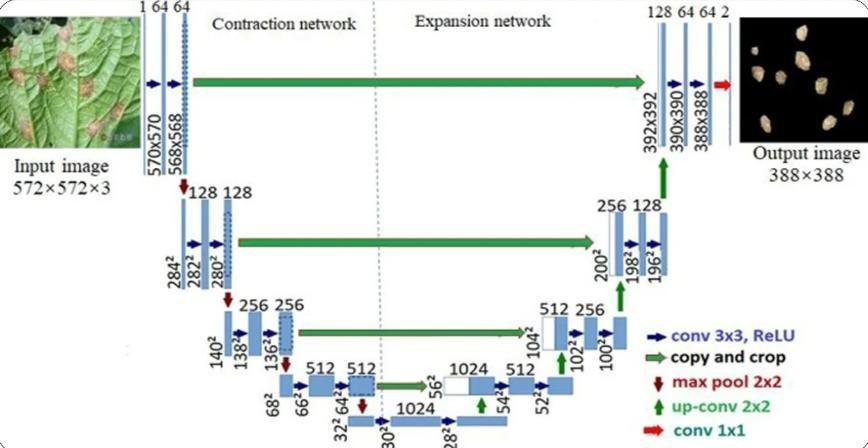
\includegraphics[width=0.8\textwidth]{images/fig11.jpg}
		\caption{ Diagrama de la arquitectura de U-Net  \cite{ultralytics_unet}.}
		\label{fig:sobel}
	\end{figure}
	
	\subsection{Aprendizaje Profundo (Deep Learning)}
	
	Una vez que la Visión por Computadora (sección 4.2) ha proporcionado las técnicas necesarias para procesar y estandarizar las imágenes digitales, el siguiente paso consiste en dotar al sistema de la capacidad de interpretar dicha información visual. Para comprender el modelo fundamental del prototipo, es indispensable explorar los fundamentos del Aprendizaje Profundo (Deep Learning).
	
	El Aprendizaje Profundo (Deep Learning) es un enfoque fundamental dentro del campo de la inteligencia artificial. Históricamente, los sistemas de inteligencia artificial se basaban en reglas lógicas explícitamente codificadas por humanos. Posteriormente, el Aprendizaje Automático (Machine Learning) permitió a los sistemas aprender a partir de datos; sin embargo, aún requería que expertos diseñaran manualmente las características (\textit{features}) que representaban la información \cite{goodfellow2016dl}.
	
	El Aprendizaje Profundo aborda esta limitación mediante modelos capaces de aprender representaciones jerárquicas de los datos. Esto permite a los sistemas construir conceptos complejos a partir de representaciones más simples, eliminando en gran medida la necesidad de diseñar características manualmente. Este enfoque ha sido clave para el desarrollo de modelos capaces de interpretar imágenes con alta precisión \cite{goodfellow2016dl,geron2019}.
	
	\subsubsection{Fundamentos de las redes neuronales artificiales}
	
	El Aprendizaje Profundo (Deep Learning) es un subcampo del Aprendizaje Automático (Machine Learning) que se basa en el uso de Redes Neuronales Artificiales (RNA). El Aprendizaje Automático describe la capacidad de un sistema para aprender a partir de datos de entrenamiento específicos de un problema, superando las limitaciones de los sistemas tradicionales en los que todo el conocimiento debía ser codificado manualmente por humanos \cite{geron2019}.
	
	Dentro del Aprendizaje Automático, la familia de las redes neuronales artificiales son de particular interés, ya que su estructura flexible permite adaptarlas a una amplia variedad de contextos. Inspiradas en el procesamiento de información en los sistemas biológicos, las RNA consisten en modelos matemáticos compuestos por unidades de procesamiento interconectadas denominadas neuronas artificiales. El estudio de esta unidad fundamental permite comprender el funcionamiento de arquitecturas más complejas \cite{geron2019}.
	
	Una neurona artificial es un modelo computacional inspirado en el comportamiento de las neuronas biológicas. Las neuronas naturales reciben señales a través de sinapsis ubicadas en las dendritas o en la membrana celular. Cuando la suma de las señales recibidas supera un determinado umbral, la neurona se activa y transmite una señal a través del axón, la cual puede propagarse hacia otras neuronas y continuar el proceso de activación en la red \cite{gershenson2003ann}.
	
	\begin{figure}[H]
		\centering
		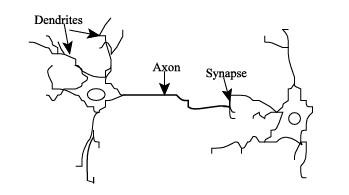
\includegraphics[width=0.6\textwidth]{images/fig12.jpg}
		\caption{ Neuronas Naturales  \cite{gershenson2003ann}.}
		\label{fig:neurona}
	\end{figure}
	
	La complejidad de las neuronas biológicas se simplifica considerablemente al modelarlas como neuronas artificiales. Estas consisten en un conjunto de entradas, análogas a las sinapsis, las cuales son multiplicadas por pesos que representan la intensidad de cada señal. Posteriormente, estas entradas ponderadas son procesadas mediante una función matemática que determina el nivel de activación de la neurona. Aunque también puede emplearse una función de salida (como la función identidad) para generar la respuesta final de la neurona, en algunos casos considerando un umbral de activación.
	
	Las Redes Neuronales Artificiales (RNA) surgen de la interconexión de múltiples neuronas artificiales, lo que permite el procesamiento de información de manera distribuida y la modelación de relaciones complejas entre los datos \cite{gershenson2003ann}.
	
	\begin{figure}[H]
		\centering
		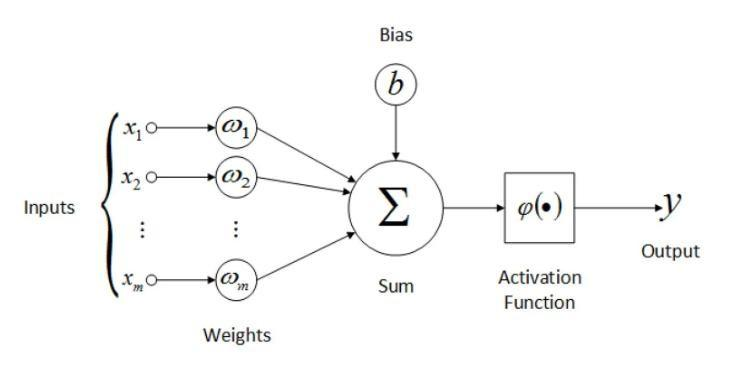
\includegraphics[width=0.8\textwidth]{images/fig13.jpg}
		\caption{ Neuronas Artificial   \cite{gershenson2003ann}.}
		\label{fig:neuronaArt}
	\end{figure}
	
	La neurona artificial es la unidad de procesamiento simple diseñada para imitar la acción de una neurona biológica. Su función es recibir múltiples señales de entrada, procesarlas de manera simple y determinar si debe generar una señal de salida \cite{zupan1994}.
	
	Sus componentes matemáticos clave son los siguientes:
	
	\begin{itemize}
		\item \textbf{Entradas ($x_i$):} Son las señales numéricas que la neurona recibe \cite{zupan1994}.
		
		\item \textbf{Pesos ($w_i$):} Son los coeficientes asociados a cada entrada. Estos representan la importancia de cada señal y son los parámetros que se aprenden en el proceso de entrenamiento \cite{zupan1994}.
		
		\item \textbf{Función de suma (Net Input):} Es la combinación lineal de las entradas ponderadas \cite{zupan1994}.
		
		\item \textbf{Sesgo ($b$):} Es un término adicional que permite ajustar el umbral de activación de la neurona. Generalmente se implementa como una entrada adicional constante igual a 1 \cite{zupan1994}.
		
		\item \textbf{Función de activación ($\varphi$):} Es una función no lineal que procesa la suma ponderada y produce la salida de la neurona \cite{zupan1994}.
		
		\item \textbf{Salida ($y$):} Es el resultado final del procesamiento realizado por la neurona.
	\end{itemize}
	
	Matemáticamente, la neurona calcula primero la suma ponderada de sus entradas más el sesgo \cite{nandy2018}:
	
	\begin{equation}
		z = \sum_{i=1}^{n} w_i x_i + b
	\end{equation}
	
	Posteriormente, se aplica la función de activación para obtener la salida:
	
	\begin{equation}
		y = \varphi(z) = \varphi\left( \sum_{i=1}^{n} w_i x_i + b \right)
	\end{equation}
	
	Las funciones de activación son esenciales para introducir no linealidad en las Redes Neuronales Artificiales, lo cual permite modelar relaciones complejas entre las entradas y salidas. Sin una función de activación no lineal, la red completa se reduciría a una transformación lineal, limitando significativamente su capacidad de representación \cite{goodfellow2016dl}. Algunas funciones comunes:
	

	
	\begin{itemize}
		\item \textbf{Lineal:}
		\begin{equation}
			f(x) = x
		\end{equation}
		Se emplea típicamente en la capa de salida para problemas de regresión.
		
		\item \textbf{Sigmoide:}
		\begin{equation}
			f(x) = \frac{1}{1 + e^{-x}}
		\end{equation}
		Produce valores en el rango $(0,1)$, siendo útil para clasificación binaria, aunque puede presentar el problema del desvanecimiento del gradiente.
		
		\item \textbf{Tangente hiperbólica (tanh):}
		\begin{equation}
			f(x) = \frac{e^{x} - e^{-x}}{e^{x} + e^{-x}}
		\end{equation}
		Su salida se encuentra en el rango $(-1,1)$, ofreciendo mejor simetría que la sigmoide, aunque también puede sufrir del problema del desvanecimiento del gradiente.
		
		\item \textbf{ReLU (Rectified Linear Unit):}
		\begin{equation}
			f(x) = \max(0, x)
		\end{equation}
		Es ampliamente utilizada en redes neuronales profundas modernas debido a su eficiencia computacional y a que reduce los problemas de saturación \cite{haykin1999}.
	\end{itemize}
	
	La arquitectura de una red neuronal artificial típica consta de al menos tres tipos de capas:
	
	\begin{itemize}
		\item \textbf{Capa de entrada:} recibe el vector de características, como los píxeles de una imagen.
		
		\item \textbf{Capas ocultas:} una o varias capas donde ocurre la transformación del espacio de características mediante pesos, sesgos y funciones de activación.
		
		\item \textbf{Capa de salida:} produce la predicción final, por ejemplo, la clase correspondiente a una seña.
	\end{itemize}
	
	Las conexiones entre capas y su organización determinan la topología de la red, la cual puede variar ampliamente dependiendo del problema a resolver \cite{haykin1999}.
	
	\begin{figure}[H]
		\centering
		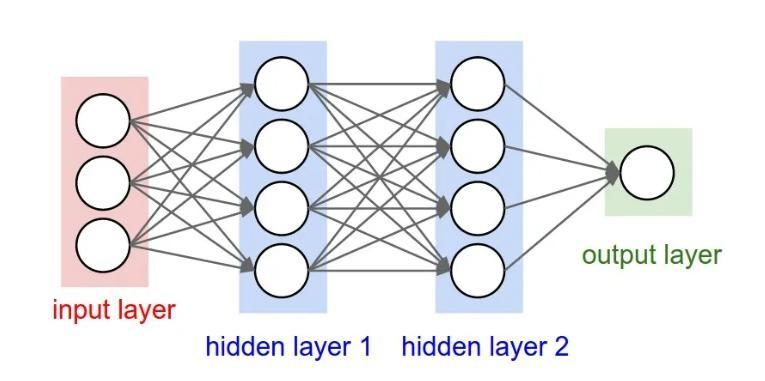
\includegraphics[width=0.8\textwidth]{images/fig15.jpg}
		\caption{ Arquitectura de una Red Neuronal Artificial.    \cite{kumar2020ann}.}
		\label{fig:arquiRNA}
	\end{figure}
	
	El entendimiento de los fundamentos de las redes neuronales artificiales es esencial para el desarrollo del presente Trabajo Terminal, ya que el reconocimiento de señas requiere que el modelo sea capaz de aprender representaciones complejas de las manos a partir de la información visual. Además, la arquitectura en capas es la base sobre la cual se construyen modelos de aprendizaje profundo, permitiendo procesar y transformar los datos de entrada en representaciones cada vez más abstractas. 
	
	\subsubsection{El proceso de entrenamiento}
	
	En la sección anterior se revisaron los fundamentos de las Redes Neuronales Artificiales (RNA); en esta sección se aborda el proceso de entrenamiento. Entrenar una red neuronal consiste en ajustar sus parámetros internos —principalmente pesos y sesgos— para que el modelo sea capaz de realizar predicciones correctas a partir de ejemplos. En este proceso la red aprende a transformar los datos de entrada en salidas adecuadas, minimizando la diferencia entre sus predicciones y los valores reales.
	
	Esta diferencia se cuantifica mediante una función de pérdida, la cual mide el desempeño del modelo en cada iteración. A medida que la red procesa más ejemplos, se espera que el valor de la pérdida disminuya, indicando una mejora en la capacidad predictiva del modelo. Un aspecto fundamental del entrenamiento es la capacidad de generalización, es decir, que el modelo funcione correctamente no solo con los datos utilizados en el entrenamiento, sino también con datos nuevos. Esto es esencial para evitar el sobreajuste, fenómeno en el cual el modelo memoriza los datos de entrenamiento sin aprender patrones generales \cite{haykin1999, goodfellow2016dl, ibm_ai_ml}.
	
	El poder de una red neuronal radica en su capacidad para aprender los valores adecuados de sus pesos y sesgos a partir de los datos. Esto se logra comparando la predicción de la red $\hat{y}$ con la etiqueta real $y$, y evaluando el error mediante una función de pérdida. En tareas de clasificación, esta función suele medir la diferencia entre la probabilidad predicha y la respuesta correcta.
	
	Para minimizar la pérdida, las redes neuronales emplean un algoritmo denominado retropropagación (\textit{backpropagation}). El proceso de entrenamiento se puede describir en cuatro etapas principales:
	
	\begin{itemize}
		\item \textbf{Pase hacia adelante (forward pass):} Las entradas se propagan a través de la red, realizando combinaciones lineales y aplicando funciones de activación no lineales, hasta obtener una predicción de salida.
		
		\item \textbf{Cálculo del error:} La función de pérdida evalúa la diferencia entre la predicción generada y el valor real.
		
		\item \textbf{Retropropagación:} El error se propaga hacia atrás a través de la red. En cada neurona, se calcula la contribución de cada peso y sesgo al error utilizando la regla de la cadena del cálculo diferencial.
		
		\item \textbf{Actualización de parámetros:} Los pesos y sesgos se ajustan en la dirección que minimiza el error, empleando algoritmos de optimización como el descenso de gradiente \cite{ibm_ai_ml}.
	\end{itemize}
	
	\begin{figure}[H]
		\centering
		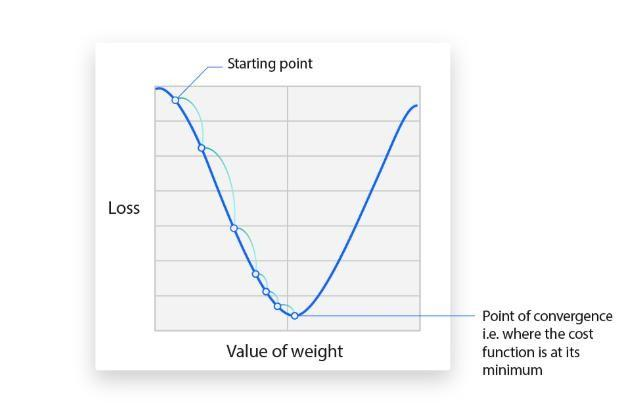
\includegraphics[width=0.6\textwidth]{images/fig16.jpg}
		\caption{ Función de pérdida.    \cite{ibm_ai_ml}.}
		\label{fig:arquiRNA}
	\end{figure}
	
	La función de pérdida es el criterio numérico que mide el error entre la salida generada por la red neuronal y el valor correcto que debería producir. Este valor sirve como guía del proceso de aprendizaje, ya que entrenar un modelo implica ajustar sus parámetros con el objetivo de minimizar dicha pérdida \cite{goodfellow2016dl}. De forma general, el ciclo de entrenamiento consiste en realizar una predicción, calcular la pérdida, estimar el error y ajustar los parámetros del modelo para mejorar su desempeño, repitiendo este proceso durante múltiples iteraciones o épocas \cite{stanford_cs231n}.
	
	La elección de la función de pérdida depende del tipo de problema a resolver. En tareas de regresión, es común emplear el Error Cuadrático Medio (MSE), el cual penaliza la diferencia entre el valor predicho y el valor real, siendo ampliamente utilizado en modelos con salidas continuas \cite{hastie2009, bishop2006}. Para problemas de clasificación multiclase, la función de pérdida más utilizada es la entropía cruzada, que mide la diferencia entre la distribución de probabilidades predicha por el modelo y la distribución verdadera es el estándar en aprendizaje profundo para este tipo de tareas \cite{hastie2009, stanford_cs231n}. 
	
	La función \textit{hinge loss} se emplea principalmente en modelos basados en márgenes, como las Máquinas de Vectores de Soporte (SVM), ya que favorece una separación clara entre clases correctas e incorrectas \cite{cs231n_linear}.
	
	La literatura coincide en que la función de pérdida no solo evalúa el desempeño del modelo, sino que también compone la fuente de la señal de aprendizaje que permite optimizar los parámetros. Esto influye directamente en la velocidad de convergencia y en la capacidad de generalización del modelo \cite{stanford_cs231n, fayaz2025}.
	
	\rowcolors{2}{rowblue}{white}
	
	\small
	\renewcommand{\arraystretch}{1.2}
	
	\begin{longtable}{|p{2.3cm}|p{3.5cm}|p{3.2cm}|p{3.5cm}|}
		\caption{Tipos de funciones de pérdida} \\
		\hline
		\rowcolor{headerblue}
		\headercell{Función de pérdida} &
		\headercell{Descripción breve} &
		\headercell{Cuándo se utiliza} &
		\headercell{Ejemplos de aplicación} \\
		\hline
		\endfirsthead
		
		\hline
		\rowcolor{headerblue}
		\headercell{Función de pérdida} &
		\headercell{Descripción breve} &
		\headercell{Cuándo se utiliza} &
		\headercell{Ejemplos de aplicación} \\
		\hline
		\endhead
		
		\rowcolors{1}{rowblue}{white}
		
		Error Cuadrático Medio (MSE) &
		Mide el promedio del cuadrado de la diferencia entre predicciones y valores reales. Penaliza fuertemente errores grandes. &
		Problemas de regresión. &
		Predicción de precios, series de tiempo, regresión lineal y redes neuronales para regresión. \\
		\hline
		
		Entropía Cruzada Categórica (Categorical Cross-Entropy) &
		Evalúa la diferencia entre la distribución de probabilidad predicha y la distribución real. &
		Clasificación multiclase con etiquetas one-hot. &
		Clasificación de imágenes, reconocimiento de objetos, clasificación de texto. \\
		\hline
		
		Entropía Cruzada Escasa (Sparse Categorical Cross-Entropy) &
		Variante de la anterior que utiliza etiquetas enteras en lugar de codificación one-hot. &
		Clasificación multiclase con muchas clases o datasets grandes. &
		Clasificación de imágenes con gran número de clases, procesamiento de lenguaje natural. \\
		\hline
		
		Binary Cross-Entropy (BCE) &
		Mide el error entre predicciones y etiquetas binarias. &
		Clasificación binaria o multietiqueta (one-vs-all). &
		Detección de spam, diagnóstico médico binario, detección de rostros vs no rostro. \\
		\hline
		
		Hinge Loss &
		Busca maximizar el margen entre clases, favoreciendo una separación clara entre clases correctas e incorrectas. &
		Modelos basados en márgenes como SVM. &
		Clasificación de dígitos, reconocimiento facial clásico, problemas con SVM. \\
		\hline
		
		Huber Loss &
		Combina MSE y MAE para ser robusta frente a valores atípicos. &
		Problemas de regresión con presencia de outliers. &
		Predicción de series ruidosas, pronósticos financieros. \\
		\hline
		
	\end{longtable}
	
	
	Ahora bien, para comprender cómo una red neuronal ajusta sus parámetros (pesos y sesgos), es necesario analizar el proceso de minimización de la función de pérdida. Para ello, se debe cuantificar cómo cambia dicha función ante pequeñas variaciones en los parámetros del modelo, lo cual se logra mediante el cálculo del gradiente.
	
	El gradiente corresponde al vector de derivadas parciales de la función de pérdida con respecto a cada uno de los parámetros del modelo. Este vector indica tanto la dirección como la magnitud del cambio necesario para reducir el error \cite{bishop2006, goodfellow2016dl}. En términos conceptuales, el gradiente permite determinar si un peso debe incrementarse o disminuirse para mejorar el desempeño de la red.
	
	La técnica computacional empleada para calcular estos gradientes de manera eficiente en redes neuronales es la retropropagación del error (\textit{backpropagation}), formalizada por Rumelhart, Hinton y Williams en 1986 \cite{rumelhart1986}. Este algoritmo se basa en la aplicación de la regla de la cadena del cálculo diferencial para propagar el error desde la capa de salida hacia las capas anteriores, permitiendo estimar la contribución de cada parámetro al error total \cite{goodfellow2016dl, rumelhart1986}.
	
	El proceso de retropropagación se lleva a cabo en dos fases principales \cite{goodfellow2016dl, geron2019}:
	
	\begin{itemize}
		\item \textbf{Propagación hacia adelante (\textit{forward pass}):} Los datos de entrada se introducen en la red y se generan las predicciones. A partir de estas, se calcula la función de pérdida comparando la salida del modelo con la etiqueta real.
		
		\item \textbf{Propagación hacia atrás (\textit{backward pass}):} El error calculado se propaga en sentido inverso a través de la red, obteniendo los gradientes de la función de pérdida con respecto a cada parámetro. Estos gradientes son utilizados por un algoritmo de optimización para actualizar los pesos y sesgos, reduciendo la pérdida en iteraciones posteriores.
	\end{itemize}
	
	\begin{figure}[H]
		\centering
		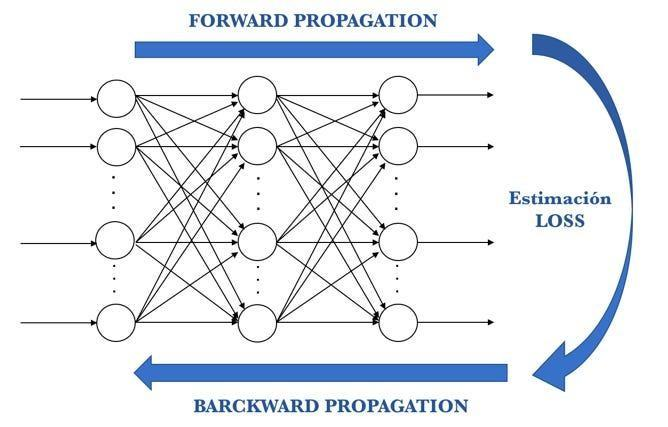
\includegraphics[width=0.5\textwidth]{images/fig17.jpg}
		\caption{ Fases principales de Backpropagation   \cite{cafeytech_nn}.}
		\label{fig:arquiRNA}
	\end{figure}
	
	La importancia del algoritmo de retropropagación radica en que permite entrenar redes neuronales profundas con un gran número de parámetros de manera computacionalmente viable, lo cual no era posible antes de su desarrollo \cite{geron2019}.
	
	La retropropagación continúa siendo el método fundamental para el entrenamiento de modelos de Deep Learning. Un ejemplo representativo es el trabajo de Krizhevsky, Sutskever y Hinton (2012), quienes entrenaron AlexNet, una de las primeras redes profundas exitosas para la clasificación de imágenes a gran escala, utilizando descenso de gradiente estocástico junto con retropropagación \cite{krizhevsky2012alexnet}. De manera más reciente, arquitecturas como ResNet, EfficientNet y modelos optimizados para dispositivos móviles siguen empleando la retropropagación como núcleo de su proceso de entrenamiento \cite{krizhevsky2012, tan2019efficientnet}. Estas arquitecturas serán analizadas con mayor detalle en secciones posteriores.
	
	Ya revisados los fundamentos del aprendizaje profundo —incluyendo el proceso de entrenamiento de una red neuronal, el papel de la función de pérdida en la medición del error y el mecanismo mediante el cual se calculan y propagan los gradientes a través del modelo (backpropagation)—, es posible comprender que estos elementos, por sí solos, no garantizan un aprendizaje eficiente. Para mejorar el desempeño del modelo, es necesario un proceso que utilice la información proporcionada por la pérdida y los gradientes para actualizar los parámetros en la dirección que reduzca el error.
	
	La optimización forma parte del componente que articula los elementos anteriores, ya que define cómo se ajustan los pesos y sesgos en el entrenamiento teniendo como objetivo minimizar la función de pérdida y lograr una convergencia efectiva del modelo \cite{goodfellow2016dl, bishop2006}.
	
	El entrenamiento de una red neuronal no se limita únicamente al cálculo del error mediante una función de pérdida ni a la obtención de los gradientes que describen la relación entre dicho error y los parámetros del modelo. Para que esta información se traduzca en aprendizaje efectivo, es necesario un proceso sistemático que utilice estos elementos para ajustar los pesos y sesgos, de tal forma que la pérdida disminuya progresivamente a lo largo de las iteraciones. Este proceso es conocido como optimización, y es un componente central del aprendizaje profundo, ya que define la manera en que los parámetros del modelo se actualizan con el objetivo de minimizar la función de pérdida y lograr una convergencia adecuada en el entrenamiento \cite{goodfellow2016dl, bishop2006, ruder2016overview}.
	
	En el del aprendizaje profundo, optimizar implica encontrar el conjunto de parámetros que produzca el mejor desempeño del modelo en la tarea asignada, lo cual equivale a buscar valores que minimicen la función de pérdida. Sin embargo, la naturaleza no lineal y de alta dimensionalidad de los modelos de redes neuronales hace que este proceso sea complejo, por lo que se requieren métodos que permitan avanzar de manera eficiente hacia soluciones adecuadas, evitando quedar atrapados en soluciones subóptimas \cite{bishop2006, goodfellow2016dl}.
	
	El método más comúnmente utilizado para guiar el proceso de optimización es el Descenso del Gradiente (\textit{Gradient Descent, GD}), el cual se basa en ajustar los parámetros del modelo en la dirección opuesta al gradiente de la función de pérdida. De manera conceptual, el gradiente indica la dirección en la que la pérdida crece más rápidamente; por lo tanto, avanzar en sentido contrario permite aproximarse a un mínimo de dicha función. En cada iteración, los parámetros se actualizan mediante pequeños ajustes en esta dirección, lo que conduce a una reducción progresiva del error en evaluaciones sucesivas del modelo \cite{geron2019}.
	
	No obstante, el descenso del gradiente en su forma básica presenta limitaciones importantes, especialmente en el caso de grandes conjuntos de datos o arquitecturas profundas, ya que requiere evaluar todo el conjunto de entrenamiento en cada actualización de los parámetros. Esto implica un alto costo computacional y tiempos de convergencia prolongados \cite{bishop2006, geron2019}.
	
	Para superar estas limitaciones, se han propuesto diversas variantes que buscan acelerar la convergencia, estabilizar el proceso de aprendizaje y mejorar el desempeño del modelo en el entrenamiento. Estas variantes introducen modificaciones en el cálculo del gradiente o en la forma en que se aplican las actualizaciones a los parámetros, y han sido fundamentales para el desarrollo del aprendizaje profundo moderno \cite{bottou2012sgd, tieleman2012rmsprop}.
	
	Una de las principales variantes es el Descenso del Gradiente Estocástico (\textit{Stochastic Gradient Descent, SGD}). A diferencia del método tradicional, SGD calcula el gradiente utilizando una sola muestra o un subconjunto reducido de datos (\textit{mini-batch}), lo que reduce significativamente el costo computacional por iteración. Además, introduce una cantidad controlada de variabilidad en el proceso de optimización, lo cual puede ayudar a evitar mínimos locales poco deseables. Sin embargo, este enfoque puede generar actualizaciones más inestables y requiere un ajuste cuidadoso de la tasa de aprendizaje para asegurar una convergencia adecuada \cite{geron2019, bottou2012sgd}.
	
	Por otro lado, el método Momentum extiende a SGD incorporando una noción de ``inercia'' en el proceso de actualización. En lugar de depender únicamente del gradiente de la iteración actual, este método acumula información de gradientes previos, lo que permite mantener una dirección de actualización más consistente. De esta forma, se suaviza la trayectoria de aprendizaje, se aceleran los avances en regiones donde el gradiente presenta una dirección sostenida y se reducen las oscilaciones en zonas con pendientes pronunciadas, favoreciendo una convergencia más estable \cite{geron2019, tieleman2012rmsprop}.
	
	Otra variante ampliamente utilizada es RMSProp, la cual introduce un mecanismo adaptativo al ajustar la magnitud de los pasos de aprendizaje en función del historial reciente de los gradientes. En particular, RMSProp normaliza la tasa de aprendizaje de cada parámetro dividiéndola por una media móvil de los cuadrados de los gradientes. Esto permite reducir la velocidad de actualización en dimensiones con gradientes elevados y aumentarla en aquellas donde los gradientes son pequeños, lo cual es útil en funciones de pérdida con curvaturas diferentes en cada dimensión, una situación común en modelos profundos \cite{bottou2012sgd, tieleman2012rmsprop}.
	
	El optimizador Adam (\textit{Adaptive Moment Estimation}) combina las ventajas de métodos como Momentum y RMSProp al estimar simultáneamente los momentos de primer orden (media de los gradientes) y de segundo orden (media de los gradientes al cuadrado). Esta estrategia permite realizar actualizaciones adaptativas para cada parámetro, manteniendo al mismo tiempo una convergencia rápida y estable. Debido a estas características, Adam se ha consolidado como uno de los optimizadores más utilizados en el aprendizaje profundo, mostrando un buen desempeño en una amplia variedad de tareas y una menor sensibilidad a la elección inicial de hiperparámetros \cite{ruder2016overview, loshchilov2019adamw}.
	
	Como evolución de este enfoque, se han propuesto variantes como AdamW, que introduce una separación explícita entre el proceso de regularización (\textit{weight decay}) y la actualización de los parámetros. Esta modificación mejora la capacidad de generalización del modelo, en particular en arquitecturas modernas de aprendizaje profundo \cite{loshchilov2019adamw}.
	
	\rowcolors{2}{rowblue}{white}
	
	\small
	\renewcommand{\arraystretch}{1.2}
		
	\begin{longtable}{|p{2.0cm}|p{3.0cm}|p{2.5cm}|p{2.5cm}|p{2.5cm}|}
		\caption{Tipos de optimizadores} \\
		\hline
		\rowcolor{headerblue}
		\headercell{Optimizador} &
		\headercell{Características principales} &
		\headercell{Ventajas} &
		\headercell{Limitaciones} &
		\headercell{Uso recomendado} \\
		\hline
		\endfirsthead
		
		\hline
		\rowcolor{headerblue}
		\headercell{Optimizador} &
		\headercell{Características principales} &
		\headercell{Ventajas} &
		\headercell{Limitaciones} &
		\headercell{Uso recomendado} \\
		\hline
		\endhead
		
		\rowcolors{1}{rowblue}{white}
		
		GD (Gradient Descent) &
		Utiliza todo el conjunto de entrenamiento para cada actualización de los parámetros. &
		Trayectoria de convergencia estable y precisa hacia el mínimo. &
		Alto costo computacional; lento en conjuntos de datos grandes. &
		Modelos pequeños o problemas teóricos. \\
		\hline
		
		SGD (Stochastic Gradient Descent) &
		Actualiza los parámetros utilizando una muestra o un mini-batch de datos. &
		Menor costo computacional por iteración; puede escapar de mínimos locales. &
		Trayectoria ruidosa; requiere ajuste fino de la tasa de aprendizaje. &
		Grandes conjuntos de datos; Deep Learning y visión por computadora. \\
		\hline
		
		Momentum &
		Incorpora una noción de ``inercia'' acumulando gradientes pasados para mantener una dirección consistente. &
		Convergencia más rápida y estable; reduce oscilaciones. &
		Puede divergir si los hiperparámetros no se ajustan adecuadamente. &
		Modelos profundos con superficies de pérdida irregulares. \\
		\hline
		
		RMSProp &
		Ajusta la tasa de aprendizaje de cada parámetro según el historial reciente de gradientes. &
		Buen desempeño en problemas no estacionarios; convergencia rápida en la práctica. &
		Puede sesgarse hacia soluciones subóptimas si no se combina con otras técnicas. &
		Redes recurrentes (RNN) y problemas con gradientes de distinta escala. \\
		\hline
		
		Adam &
		Combina las ventajas de Momentum y RMSProp mediante actualizaciones adaptativas de los parámetros. &
		Rápido, estable y con buen desempeño en la mayoría de tareas. &
		Puede sobreajustar si no se aplica regularización adecuada. &
		Uso general en Deep Learning: visión por computadora, NLP y audio. \\
		\hline
		
	\end{longtable}
	
	La correcta selección del algoritmo de optimización es importante para lograr un entrenamiento eficiente y una convergencia adecuada del modelo. Si bien existen múltiples alternativas, cada una con ventajas y limitaciones, optimizadores adaptativos como Adam han demostrado un desempeño consistente en aplicaciones de visión por computadora y reconocimiento de patrones, por lo que se han consolidado como una opción común en el ámbito del aprendizaje profundo moderno \cite{ruder2016overview, loshchilov2019adamw, tieleman2012rmsprop}. En el presente trabajo, se empleará un optimizador perteneciente a esta familia, cuya selección y configuración específica se detallarán en el capítulo correspondiente.
	
	Como se mencionó anteriormente, el proceso de entrenamiento de una red neuronal no depende únicamente de la arquitectura del modelo o de la función de pérdida utilizada, sino también de un conjunto de valores previamente definidos conocidos como hiperparámetros. A diferencia de los parámetros internos de la red, como los pesos y sesgos, que se ajustan automáticamente en el proceso del aprendizaje, los hiperparámetros son configuraciones externas que determinan cómo se llevará a cabo dicho proceso. Su correcta selección influye directamente en la velocidad de convergencia, la estabilidad del entrenamiento y la capacidad del modelo para generalizar adecuadamente a nuevos datos \cite{bishop2006, goodfellow2016dl}.
	
	La elección de hiperparámetros conforma una de las etapas más críticas del modelado, ya que combinaciones inadecuadas pueden conducir a modelos incapaces de aprender patrones relevantes, entrenamientos inestables o sistemas que memorizan los datos sin generalizar adecuadamente \cite{chollet2021, geron2019}. En consecuencia, comprender el rol de los principales hiperparámetros es importante para fundamentar decisiones posteriores.
	
	A continuación, se presentan los hiperparámetros más relevantes que se consideran de manera general en el entrenamiento de modelos de aprendizaje profundo.
	
	\begin{itemize}
		
		\item \textbf{Tasa de aprendizaje (\textit{Learning Rate}):} es uno de los hiperparámetros más influyentes, ya que controla el tamaño del paso con el que el algoritmo de optimización actualiza los pesos en el descenso del gradiente \cite{goodfellow2016dl}. Si su valor es demasiado alto, el entrenamiento puede volverse inestable y divergir; mientras que un valor excesivamente bajo puede provocar una convergencia lenta o que el modelo quede atrapado en mínimos locales subóptimos \cite{smith2018}. Debido a su impacto, la literatura propone estrategias como el ajuste manual, el uso de métodos adaptativos o esquemas de programación (\textit{schedulers}) para modificar la tasa de aprendizaje en el entrenamiento.
		
		\item \textbf{Tamaño del lote (\textit{Batch Size}):} define el número de muestras utilizadas para realizar una actualización de los parámetros del modelo. Su elección influye tanto en el desempeño computacional como en la estabilidad del gradiente. Lotes pequeños generan actualizaciones más ruidosas, lo que puede favorecer la generalización, mientras que lotes grandes producen gradientes más estables y eficientes computacionalmente, aunque con el riesgo de converger a soluciones menos óptimas \cite{keskar2017, goyal2017}. En la práctica, se busca un equilibrio entre estabilidad, tiempo de entrenamiento y uso de memoria disponible \cite{goodfellow2016dl}.
		
		\item \textbf{Número de épocas (\textit{Epochs}):} representa el número de veces que el modelo recorre el conjunto completo de entrenamiento. Un número insuficiente de épocas puede impedir que el modelo aprenda adecuadamente (\textit{underfitting}), mientras que un número excesivo incrementa el riesgo de sobreajuste (\textit{overfitting}) \cite{bishop2006, ng2020}. La selección adecuada de este parámetro suele basarse en el monitoreo de la pérdida y las métricas en un conjunto de validación.
		
		\item \textbf{Optimizador:} es el método utilizado para ajustar los pesos del modelo en función del gradiente de la función de pérdida. Este es un hiperparámetro esencial, ya que diferentes algoritmos presentan comportamientos distintos en términos de velocidad de convergencia, estabilidad y capacidad para escapar de mínimos locales \cite{shalev2014}. Entre los más utilizados se encuentran SGD, RMSProp y Adam, cuyo análisis fue abordado previamente en la sección correspondiente a métodos de optimización.
		
		\item \textbf{Regularización:} es un conjunto de técnicas cuyo objetivo es mejorar la capacidad de generalización del modelo mediante penalizaciones que limitan su complejidad. Una regularización adecuada reduce el riesgo de sobreajuste al evitar que los pesos crezcan de manera desproporcionada o que el modelo memorice los datos de entrenamiento \cite{bishop2006}. Entre las técnicas más comunes se encuentran la regularización L1 y L2. La regularización L1 promueve la esparsidad en los parámetros, mientras que L2 distribuye la penalización de forma más uniforme entre los pesos del modelo \cite{krogh1992, zhang2019}.
		
		\item \textbf{Pesos de clase (\textit{Class Weights}):} en problemas de clasificación con clases desbalanceadas, permiten asignar mayor importancia a las clases minoritarias, evitando que el modelo favorezca las clases más representadas \cite{he2009}. Esta técnica ajusta la función de pérdida para que los errores en clases poco frecuentes tengan un mayor impacto en la actualización de los parámetros, mejorando la equidad del modelo y su capacidad de generalización \cite{japkowicz2002}.
		
	\end{itemize}
	
	
	\rowcolors{2}{rowblue}{white}
	
	\small
	\renewcommand{\arraystretch}{1.2}
	
	\begin{longtable}{|p{2.3cm}|p{3.0cm}|p{3.0cm}|p{3.0cm}|}
		\caption{Diferencias entre hiperparámetros} \\
		\hline
		\rowcolor{headerblue}
		\headercell{Hiperparámetro} &
		\headercell{Propósito} &
		\headercell{Consecuencia de mala elección} &
		\headercell{¿Se puede anticipar el efecto sin experimentar?} \\
		\hline
		\endfirsthead
		
		\hline
		\rowcolor{headerblue}
		\headercell{Hiperparámetro} &
		\headercell{Propósito} &
		\headercell{Consecuencia de mala elección} &
		\headercell{¿Se puede anticipar el efecto sin experimentar?} \\
		\hline
		\endhead
		
		\rowcolors{1}{rowblue}{white}
		
		Learning Rate &
		Controla el tamaño del paso con el que se actualizan los pesos. &
		Divergencia, estancamiento o convergencia lenta. &
		Parcialmente. Se conocen tendencias teóricas, pero el valor óptimo suele requerir experimentación. \\
		\hline
		
		Batch Size &
		Define cuántas muestras se utilizan para actualizar los pesos en cada iteración. &
		Gradientes ruidosos o convergencia hacia soluciones menos óptimas. &
		Parcialmente. Su efecto es conocido teóricamente, pero depende del dataset y del hardware. \\
		\hline
		
		Número de épocas &
		Determina cuántas veces el modelo recorre el conjunto completo de entrenamiento. &
		Underfitting o overfitting. &
		No. Generalmente requiere monitoreo del entrenamiento para su correcta selección. \\
		\hline
		
		Optimizador &
		Define la estrategia para actualizar los pesos utilizando el gradiente. &
		Entrenamiento lento, inestable o mala convergencia. &
		Parcialmente. Existen guías teóricas, pero la mejor opción depende del problema. \\
		\hline
		
		Regularización &
		Limita la complejidad del modelo para mejorar su capacidad de generalización. &
		Sobreajuste o incapacidad para generalizar correctamente. &
		Sí a nivel teórico, aunque la magnitud óptima requiere experimentación. \\
		\hline
		
		Class Weights &
		Compensa el desbalance de clases asignando mayor peso a las clases minoritarias. &
		Modelo sesgado hacia las clases mayoritarias. &
		Sí en la mayoría de los casos; su uso es recomendable cuando existe desbalance en los datos. \\
		\hline
		
	\end{longtable}
	
	Uno de los principales objetivos en el entrenamiento es lograr que el modelo no solo aprenda correctamente los patrones presentes en los datos de entrenamiento, sino que también sea capaz de generalizar dicho conocimiento a datos no vistos. De esta manera se identifican dos problemas característicos que afectan la calidad del aprendizaje: el \textit{underfitting} (subajuste) y el \textit{overfitting} (sobreajuste) \cite{goodfellow2016dl, geron2019}.
	
	El \textit{underfitting} ocurre cuando el modelo no logra aprender adecuadamente la estructura de los datos. Como consecuencia, presenta un alto nivel de error incluso sobre el conjunto de entrenamiento. Este problema suele estar asociado con modelos de baja capacidad representativa (por ejemplo, con pocas capas o neuronas), un entrenamiento insuficiente o una selección inadecuada de hiperparámetros \cite{goodfellow2016dl}. En general, un modelo subajustado presenta un bajo desempeño tanto en el conjunto de entrenamiento como en el de validación, lo que indica que no ha capturado la complejidad del problema.
	
	Por otro lado, el \textit{overfitting} se presenta cuando el modelo aprende en exceso los detalles y el ruido del conjunto de entrenamiento, perdiendo su capacidad de generalización frente a nuevos datos \cite{goodfellow2016dl, hastie2009}. En este caso, el modelo obtiene un desempeño muy alto en el conjunto de entrenamiento, pero presenta resultados deficientes en validación o prueba. De acuerdo con Hastie \cite{hastie2009}, este fenómeno refleja un modelo con alta varianza, lo que conduce a predicciones inconsistentes fuera del conjunto de entrenamiento.
	
	La detección de \textit{underfitting} y \textit{overfitting} suele realizarse mediante el análisis comparativo de las métricas de entrenamiento y validación a lo largo de las épocas \cite{geron2019}. El subajuste se asocia con pérdidas elevadas y baja precisión en ambos conjuntos; mientras que el sobreajuste se identifica cuando la pérdida en entrenamiento continúa disminuyendo, pero la pérdida en validación comienza a incrementarse, generando una brecha creciente entre ambas curvas. Este análisis permite diagnosticar el comportamiento del modelo incluso antes de aplicar técnicas de corrección.
	
	\rowcolors{2}{rowblue}{white}
	
	\small
	\renewcommand{\arraystretch}{1.2}
	
	\begin{longtable}{|p{4.0cm}|p{3.5cm}|p{3.5cm}|}
		\caption{Comparación entre underfitting y overfitting} \\
		\hline
		\rowcolor{headerblue}
		\headercell{Característica} &
		\headercell{Underfitting} &
		\headercell{Overfitting} \\
		\hline
		\endfirsthead
		
		\hline
		\rowcolor{headerblue}
		\headercell{Característica} &
		\headercell{Underfitting} &
		\headercell{Overfitting} \\
		\hline
		\endhead
		
		\rowcolors{1}{rowblue}{white}
		
		Aprendizaje del modelo &
		Insuficiente &
		Excesivo (incluye ruido) \\
		\hline
		
		Desempeño en entrenamiento &
		Bajo &
		Muy alto \\
		\hline
		
		Desempeño en validación/prueba &
		Bajo &
		Bajo \\
		\hline
		
		Causa principal &
		Modelo poco complejo o mal entrenado &
		Modelo demasiado complejo o entrenado en exceso \\
		\hline
		
		Capacidad de generalización &
		Deficiente &
		Deficiente \\
		\hline
		
	\end{longtable}
	
	\begin{flushleft}
		Un ejemplo conceptual que ilustra estos comportamientos es el ajuste de un modelo de clasificación de imágenes. Si el modelo es demasiado simple o se entrena durante pocas épocas, no logrará aprender las características distintivas de cada clase (\textit{underfitting}). Por el contrario, si el modelo es excesivamente complejo o se entrena en exceso, tenderá a memorizar las imágenes del conjunto de entrenamiento, fallando al clasificar correctamente datos nuevos (\textit{overfitting}) \cite{goodfellow2016dl, chollet2021, geron2019}.
		
		La comprensión de estos fenómenos es importante, ya que condiciona la selección y ajuste de hiperparámetros, así como la aplicación de estrategias preventivas que permitan mejorar la capacidad de generalización del modelo. Las principales técnicas teóricas para mitigar el \textit{overfitting} se presentan a continuación \cite{hinton2012}.
		
		Dado que el \textit{overfitting} limita la capacidad del modelo para generalizar a datos no vistos, diversos autores han propuesto estrategias que buscan reducir la complejidad efectiva del modelo, promoviendo representaciones más robustas de los patrones relevantes \cite{goodfellow2016dl, bishop2006}.
		
		\textbf{Regularización (L1 y L2).} La regularización consiste en añadir un término de penalización a la función de pérdida con la finalidad de restringir la magnitud de los pesos del modelo y evitar que éste se ajuste excesivamente a los datos de entrenamiento \cite{goodfellow2016dl}. La regularización L1 promueve la esparsidad en los parámetros al forzar algunos pesos a cero, favoreciendo la selección de características relevantes. Por su parte, la regularización L2 aplica una penalización cuadrática sobre los pesos, reduciendo su magnitud de forma más uniforme. Ambas técnicas contribuyen a mejorar la capacidad de generalización del modelo, siendo L2 la más utilizada en redes neuronales profundas debido a su estabilidad durante el entrenamiento \cite{krogh1992}.
		
		\textbf{Dropout.} Es una técnica propuesta por Hinton que consiste en desactivar aleatoriamente un porcentaje de neuronas en cada iteración del entrenamiento \cite{srivastava2014}. Este mecanismo evita que las neuronas dependan excesivamente de otras específicas y fomenta la creación de representaciones distribuidas. Desde un punto de vista teórico, el \textit{dropout} puede interpretarse como un ensamble de múltiples modelos, lo que mejora la generalización y reduce el riesgo de sobreajuste \cite{goodfellow2016dl}.
		
		\textbf{Early Stopping.} Esta técnica consiste en detener el entrenamiento cuando el desempeño del modelo en el conjunto de validación deja de mejorar en cierto número de iteraciones. Su trabajo es evitar que el modelo continúe ajustándose al ruido del conjunto de entrenamiento una vez alcanzado el punto óptimo de generalización. Su aplicación requiere monitorear la pérdida de validación y definir un criterio de paciencia adecuado \cite{hinton2012}.
		
		\textbf{Data Augmentation.} Consiste en generar nuevas muestras a partir de los datos existentes mediante transformaciones como rotaciones, reflejos, cambios de iluminación o escalado, sin modificar la etiqueta original \cite{geron2019}. De acuerdo con Shorten y Khoshgoftaar \cite{shorten2019}, esta técnica incrementa la diversidad del conjunto de entrenamiento, dificultando la memorización de los datos y promoviendo un aprendizaje más robusto. En visión por computadora, es una de las estrategias más efectivas cuando la cantidad de datos disponibles es limitada.
		
		\textbf{Validación Cruzada.} Esta técnica divide el conjunto de datos en múltiples subconjuntos para entrenar y evaluar el modelo en diferentes particiones, reduciendo el sesgo asociado a una única división entrenamiento--validación. Aunque es más común en modelos clásicos de aprendizaje automático, también resulta útil en redes neuronales cuando el conjunto de datos es reducido y se busca una evaluación más fiable del desempeño del modelo \cite{hastie2009}.
	\end{flushleft}
	
	\rowcolors{2}{rowblue}{white}
	
	\small
	\renewcommand{\arraystretch}{1.2}
	
	\begin{longtable}{|p{2.5cm}|p{3.2cm}|p{2.8cm}|p{2.8cm}|}
		\caption{Técnicas para reducir el overfitting} \\
		\hline
		\rowcolor{headerblue}
		\headercell{Técnica} &
		\headercell{Principio de funcionamiento} &
		\headercell{Ventaja principal} &
		\headercell{Limitación} \\
		\hline
		\endfirsthead
		
		\hline
		\rowcolor{headerblue}
		\headercell{Técnica} &
		\headercell{Principio de funcionamiento} &
		\headercell{Ventaja principal} &
		\headercell{Limitación} \\
		\hline
		\endhead
		
		\rowcolors{1}{rowblue}{white}
		
		Regularización L1/L2 &
		Penaliza la magnitud de los pesos del modelo. &
		Mejora la capacidad de generalización. &
		Requiere un ajuste adecuado del parámetro de regularización. \\
		\hline
		
		Dropout &
		Desactiva neuronas de manera aleatoria en el proceso del entrenamiento. &
		Evita la co-adaptación y reduce la memorización. &
		Un uso excesivo puede ralentizar el entrenamiento. \\
		\hline
		
		Early Stopping &
		Detiene el entrenamiento al detectar deterioro en la validación. &
		Fácil de implementar y eficiente. &
		Requiere monitoreo adecuado del proceso de entrenamiento. \\
		\hline
		
		Data Augmentation &
		Aumenta la variabilidad del dataset mediante transformaciones. &
		Muy eficaz cuando se dispone de pocos datos. &
		Puede alterar la semántica si se aplica incorrectamente. \\
		\hline
		
		Validación Cruzada (Cross-Validation) &
		Evalúa el modelo en múltiples particiones del dataset. &
		Reduce el sesgo en la evaluación. &
		Alto costo computacional. \\
		\hline
		
	\end{longtable}
	Estas técnicas conforman la base teórica empleada en la práctica para mejorar la capacidad de generalización de los modelos. Su adecuada selección y combinación dependen de la naturaleza del problema, el tamaño del conjunto de datos y la complejidad del modelo utilizado \cite{geron2019}.
	
	Los conceptos revisados en esta sección —entrenamiento de redes neuronales, función de pérdida, retropropagación, optimización, hiperparámetros y el equilibrio entre \textit{underfitting} y \textit{overfitting}— conforman el fundamento teórico necesario para comprender cómo los modelos de aprendizaje profundo adquieren la capacidad de generalizar a datos no vistos.
	
	
	\subsubsection{Redes neuronales convolucionales (CNN)}
	
	El origen de las Redes Neuronales Convolucionales (CNN) se remonta al trabajo de Yann LeCun a finales de la década de 1980, cuando integró el algoritmo de retropropagación con operaciones de convolución para el reconocimiento automático de patrones \cite{lecun1989}. Este avance dio lugar a la arquitectura LeNet-5, presentada por LeCun et al. en 1998, la cual destacó por su éxito en el reconocimiento de dígitos escritos a mano y fue implementada en sistemas reales como el del Servicio Postal de los Estados Unidos \cite{lecun1998}. Sin embargo, el uso de CNN no se popularizó de inmediato debido a las limitaciones computacionales de la época.
	
	El resurgimiento de las CNN se produjo en 2012 con AlexNet, desarrollada por Krizhevsky, Sutskever y Hinton, la cual logró una reducción significativa del error en la competencia ImageNet, superando ampliamente a los métodos tradicionales de visión por computadora. Este resultado marcó un punto de inflexión y consolidó a las CNN como el enfoque predominante para tareas de clasificación de imágenes, detección y reconocimiento de objetos \cite{krizhevsky2012alexnet}.
	
	De manera general, una red neuronal artificial (RNA) tradicional está compuesta por neuronas organizadas en capas completamente conectadas (\textit{fully-connected}), donde cada neurona transmite su salida a todas las neuronas de la siguiente capa. Si bien este tipo de arquitectura es capaz de modelar relaciones no lineales complejas, resulta ineficiente para el procesamiento de imágenes, ya que implica un número elevado de parámetros y no preserva la estructura espacial de los datos. Estas limitaciones motivaron el desarrollo de arquitecturas especializadas como las CNN, diseñadas específicamente para explotar la naturaleza espacial de las imágenes \cite{haykin1999}.
	
	Una Red Neuronal Convolucional (CNN) es un modelo especializado para el procesamiento de datos con estructura espacial, como las imágenes. Estas redes emplean operaciones de convolución que permiten analizar regiones locales de la imagen preservando la relación entre los píxeles, lo cual facilita la detección y el aprendizaje de patrones visuales como bordes, formas y texturas \cite{oshea2015}. Las CNN reducen significativamente la cantidad de parámetros mediante el uso de filtros compartidos (\textit{weight sharing}), lo que las hace más eficientes, menos propensas al sobreajuste y más adecuadas para el procesamiento de información visual en comparación con las redes densas tradicionales \cite{oshea2015}.
	
	La arquitectura de una CNN se compone, de manera general, de dos etapas principales: extracción de características y clasificación. Esta organización permite que el modelo procese las imágenes preservando su estructura espacial y, posteriormente, utilice la información aprendida para asignar una etiqueta o categoría a la entrada. A diferencia de las redes neuronales completamente conectadas, donde cada neurona se relaciona con todas las unidades de la capa anterior, las CNN aprovechan la localización espacial de los píxeles para aprender patrones de forma jerárquica y eficiente \cite{goodfellow2016dl, lecun1995}.
	
	En la primera etapa, denominada extracción de características, la red aplica de forma secuencial operaciones de convolución, funciones de activación y, en muchos casos, operaciones de \textit{pooling}. Las capas convolucionales utilizan filtros (o \textit{kernels}) que recorren la imagen con el fin de detectar patrones locales, como bordes, esquinas o texturas. Conforme aumenta la profundidad de la red, las capas subsiguientes aprenden representaciones más complejas y abstractas, pasando de características simples a descriptores de mayor nivel semántico. Por su parte, el \textit{pooling} reduce progresivamente la dimensionalidad de los mapas de características, conservando la información más relevante y disminuyendo el costo computacional \cite{gibson2015}.
	
	\begin{figure}[H]
		\centering
		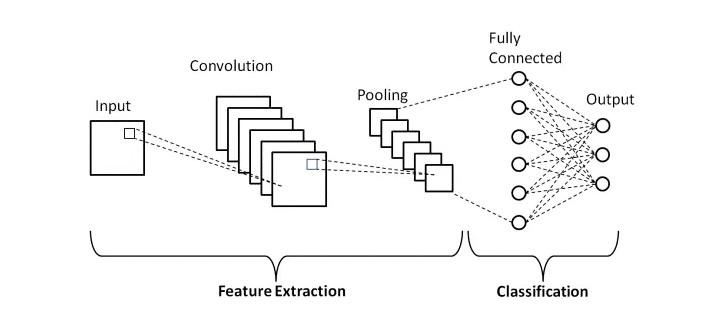
\includegraphics[width=0.5\textwidth]{images/fig18.jpg}
		\caption{ Arquitectura de Red Neuronal Convolucional.  \cite{dai2021cnn}.}
		\label{fig:arquiCNN}
	\end{figure}
	
	La segunda etapa corresponde a la clasificación. Despues de obtener los mapas de características, estos se transforman en un vector unidimensional mediante una operación de aplanado (\textit{flattening}) y se introducen en una o más capas totalmente conectadas (\textit{fully connected}). Estas capas actúan como un clasificador que combina la información extraída para determinar la clase final de la imagen. En problemas de clasificación multiclase, la capa de salida suele emplear la función \textit{softmax}, la cual permite generar probabilidades normalizadas asociadas a cada categoría \cite{goodfellow2016dl, bishop2006}.
	
	Esta arquitectura modular permite automatizar el proceso de aprendizaje de características, eliminando la necesidad de ingeniería manual de atributos, como ocurría en los enfoques tradicionales de visión por computadora. Gracias a su capacidad para aprender representaciones invariantes y altamente discriminativas, las CNN se han consolidado como el enfoque dominante en aplicaciones como reconocimiento facial, clasificación de objetos, conducción autónoma y reconocimiento de señas, donde la preservación de patrones visuales es fundamental \cite{lecun1995, lecun2015deep}.
	
	A continuación, se describen los componentes fundamentales que conforman la etapa de extracción de características, comenzando por la operación de convolución, considerada el núcleo de este proceso.
	
	La operación de convolución representa el elemento central de las Redes Neuronales Convolucionales, ya que permite procesar datos con estructura espacial de forma más eficiente que las redes neuronales tradicionales. En una red completamente conectada, cada neurona se enlaza con todas las entradas de la capa anterior, lo que implica un número elevado de parámetros y provoca la pérdida de la estructura espacial entre los píxeles. Esta característica limita la capacidad del modelo para reconocer patrones visuales locales, además de incrementar el riesgo de sobreajuste y el costo computacional \cite{goodfellow2016dl}.
	
	La convolución introduce los conceptos de campos receptivos locales (\textit{local receptive fields}) y compartición de pesos (\textit{weight sharing}), permitiendo que la red aprenda patrones visuales mediante filtros que se desplazan sobre regiones de la imagen. De esta manera, la CNN aprende de forma jerárquica: inicialmente detecta características simples como bordes y contornos; posteriormente identifica patrones más complejos como formas y texturas; y, en capas más profundas, construye representaciones de alto nivel semántico \cite{oshea2015}. Este enfoque reduce considerablemente el número de parámetros y preserva la estructura espacial de los datos, lo que hace a las CNN adecuadas para el procesamiento de imágenes \cite{lecun2015deep, dai2021cnn}.
	
	Una imagen digital puede representarse como un tensor. En el caso de una imagen RGB, se emplean tres canales (rojo, verde y azul), cada uno representado por una matriz de tamaño $H \times W$. Por tanto, una imagen de dimensiones $H \times W \times 3$ puede modelarse como un tensor tridimensional, donde la profundidad corresponde al número de canales. Cuando una CNN procesa esta imagen, los filtros convolucionales también poseen una profundidad equivalente al número de canales, de modo que puedan capturar relaciones entre ellos \cite{oshea2015, albawi2017}. Esta representación tensorial permite que el modelo procese de forma conjunta la información cromática y espacial presente en la imagen.
	
	\subsubsection*{Definición matemática de la convolución}
	
	La operación de convolución en dos dimensiones entre una imagen de entrada $I$ y un filtro o \textit{kernel} $K$ puede expresarse como \cite{dai2021cnn}:
	
	\begin{equation}
		S(i, j) = \sum_{m=0}^{M-1} \sum_{n=0}^{N-1} I(i + m, j + n) \cdot K(m, n)
	\end{equation}
	
	donde $S(i, j)$ representa el valor obtenido en la posición $(i, j)$ del mapa de características resultante; $I$ es la imagen de entrada; y $K$ es el kernel de tamaño $M \times N$. Esta operación consiste en realizar multiplicaciones elemento a elemento entre una región local de la imagen y el filtro, seguidas de una suma acumulativa.
	
	Para imágenes multicanal, la convolución se extiende a la tercera dimensión, de modo que el filtro cubre simultáneamente todos los canales. El resultado final se obtiene mediante la suma de las convoluciones individuales realizadas en cada canal \cite{dai2021cnn, albawi2017}.
	
	El resultado de esta operación es un mapa de características (\textit{feature map}), el cual resalta la presencia de patrones aprendidos por el filtro en la imagen. A medida que se apilan múltiples capas convolucionales, las representaciones se vuelven progresivamente más abstractas, permitiendo que la CNN aprenda características relevantes para tareas de clasificación, detección o reconocimiento \cite{dai2021cnn}.
	
	
	\begin{figure}[H]
		\centering
		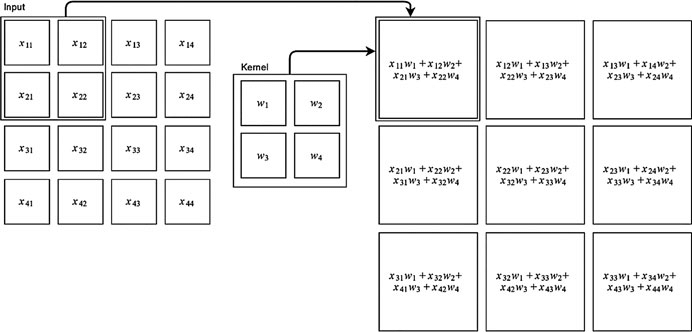
\includegraphics[width=0.8\textwidth]{images/fig19.jpg}
		\caption{ Operación de Convolución y Mapa de Características.  \cite{montesinos2022conv}.}
		\label{fig:convolucion}
	\end{figure}
	
	En resumen, la convolución proporciona a las CNN la capacidad de aprender representaciones espaciales con un número reducido de parámetros, preservando la estructura visual de la imagen y facilitando la extracción progresiva de rasgos relevantes. Esta propiedad es importante en tareas de visión por computadora, como el reconocimiento de señas, donde es necesario identificar patrones sutiles y variaciones en la forma de las manos.
	
	Las funciones de activación desempeñan un papel fundamental en la etapa de extracción de características dentro de una Red Neuronal Convolucional (CNN). Estas funciones introducen no linealidad en los mapas de características generados por la operación de convolución, permitiendo que la red aprenda relaciones complejas presentes en la imagen. Sin una función de activación, cada capa convolucional sería una transformación estrictamente lineal, por lo que múltiples capas apiladas serían equivalentes a una sola transformación lineal, limitando severamente la capacidad del modelo para aprender patrones relevantes \cite{goodfellow2016dl}.
	
	En esta etapa, la activación se aplica punto a punto sobre el mapa de características generado por la convolución. Esto permite suprimir valores irrelevantes y resaltar aquellos que contienen información discriminante, favoreciendo la representación progresiva de patrones locales que se vuelven más abstractos en capas profundas \cite{goodfellow2016dl}.
	
	Las primeras arquitecturas de redes neuronales empleaban funciones de activación suaves como la sigmoide:
	\begin{equation}
		\sigma(x) = \frac{1}{1 + e^{-x}}
	\end{equation}
	
	y la tangente hiperbólica:
	\begin{equation}
		\tanh(x) = \frac{e^{x} - e^{-x}}{e^{x} + e^{-x}}
	\end{equation}
	
	Estas funciones permiten modelar relaciones no lineales y fueron ampliamente utilizadas en los primeros modelos de reconocimiento de patrones \cite{haykin1999}. Sin embargo, presentan regiones de saturación donde el gradiente tiende a cero, generando el conocido problema del \textit{vanishing gradient}, lo cual dificulta el entrenamiento de redes profundas \cite{hochreiter1998}. Por este motivo, su uso en CNN modernas es limitado.
	
	El desarrollo de la función Rectified Linear Unit (ReLU) representó un avance significativo en el entrenamiento de modelos profundos. Definida como:
	
	\begin{equation}
		\text{ReLU}(x) = \max(0, x)
	\end{equation}
	
	esta función elimina la saturación en la región positiva, manteniendo un gradiente constante y permitiendo entrenar redes más profundas con mayor estabilidad. Nair y Hinton demostraron que ReLU mejora la propagación del gradiente y acelera la convergencia del modelo \cite{nair2010}.
	
	ReLU se popularizó tras su uso en AlexNet, modelo que marcó un punto de inflexión en el desafío ImageNet al reducir significativamente el error de clasificación \cite{krizhevsky2012alexnet}. Esta función de activación se ha convertido en un estándar debido a su simplicidad computacional, su eficiencia en el entrenamiento y su capacidad para mitigar el problema del desvanecimiento del gradiente \cite{goodfellow2016dl}.  Esta activación se convirtió en estándar por varias razones:
	
	\begin{itemize}
		\item Facilita la propagación del gradiente en redes profundas.
		\item No presenta saturación para valores positivos.
		\item Genera activaciones dispersas (\textit{sparsity}) que favorecen la eficiencia.
		\item Es computacionalmente simple y rápida de evaluar.
		\item Ha demostrado resultados superiores en múltiples arquitecturas como VGG, ResNet, MobileNet y EfficientNet.
	\end{itemize}
	
	Estos factores hacen que ReLU sea la función de activación preferida en la etapa de extracción de características dentro de las CNN contemporáneas.
	
	Tras la aplicación de la función de activación, los mapas de características resultantes contienen respuestas no lineales que destacan las regiones donde los filtros convolucionales han identificado patrones relevantes. Sin embargo, estas activaciones suelen presentar redundancia espacial y variaciones locales de intensidad que no necesariamente aportan información adicional. Para consolidar dichas respuestas y obtener representaciones más compactas y robustas, las CNN incorporan una etapa de agrupación o \textit{pooling}, la cual resume la información dentro de regiones locales y proporciona invariancia ante pequeñas traslaciones o deformaciones en la imagen \cite{goodfellow2016dl}.
	
	De este modo, el flujo convolución $\rightarrow$ activación $\rightarrow$ \textit{pooling} es el  bloque funcional clave en la extracción jerárquica de características, permitiendo que las redes incrementen su capacidad representacional mientras mantienen la eficiencia computacional y la estabilidad del aprendizaje \cite{scherer2010}.
	
	El \textit{pooling}, también denominado submuestreo espacial, es una operación fundamental dentro de la etapa de extracción de características en una CNN. Su propósito principal es reducir la dimensionalidad espacial de los mapas de características generados por la convolución, preservando la información más relevante del patrón visual. Esta operación permite que la red sea más eficiente, reduzca la cantidad de parámetros en capas posteriores y obtenga representaciones más robustas ante pequeñas transformaciones espaciales \cite{goodfellow2016dl}.
	
	Formalmente, el \textit{pooling} opera mediante una ventana local $\Omega$ de tamaño $K \times K$, la cual se desplaza con un \textit{stride} definido sobre el mapa de características $x$. Para cada posición $(i, j)$, el valor de salida se obtiene mediante la aplicación de una función de agregación $f(\cdot)$:
	
	\begin{equation}
		y(i,j) = f \big( x(p,q) \; | \; (p,q) \in \Omega_{i,j} \big)
	\end{equation}
	
	donde $\Omega_{i,j}$ representa la región local de entrada asociada a la posición $(i,j)$ en el mapa de salida.
	
	Dependiendo de la función de agregación $f$, se obtienen distintas variantes de \textit{pooling}, siendo las más comunes:
	
	\begin{itemize}
		\item \textbf{Max Pooling:} selecciona el valor máximo dentro de la región local.
		\item \textbf{Average Pooling:} calcula el promedio de los valores dentro de la región.
	\end{itemize}
	
	Estas operaciones permiten reducir la dimensionalidad espacial mientras conservan la información más relevante, contribuyendo a mejorar la capacidad de generalización del modelo \cite{scherer2010}.
	
	\begin{figure}[H]
		\centering
		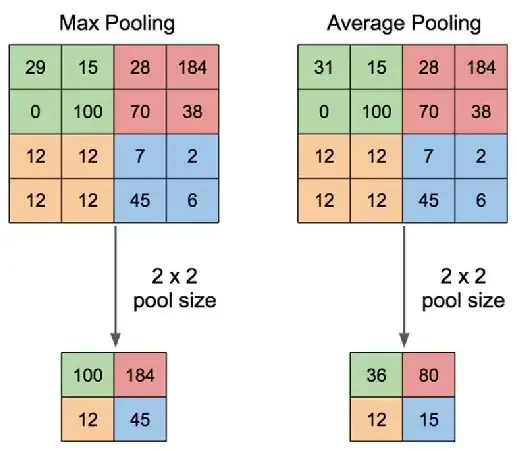
\includegraphics[width=0.8\textwidth]{images/fig20.png}
		\caption{ Max Pooling y Average Pooling.  \cite{salmiah2019cnn}.}
		\label{fig:pooling}
	\end{figure}
	
	Históricamente, el \textit{pooling} tiene sus raíces en el modelo Neocognitron de Fukushima, considerado un precursor conceptual de las CNN actuales. En este modelo se empleaba un mecanismo denominado \textit{S-cells}, el cual combinaba información local para generar invariancia ante pequeñas transformaciones espaciales \cite{fukushima1980}. Posteriormente, con la aparición de LeNet-5, el \textit{pooling} (entonces denominado \textit{subsampling}) se formalizó como una operación explícita que complementaba la convolución y permitía la reducción progresiva de la dimensionalidad espacial en redes jerárquicas \cite{lecun1998}.
	
	Con el desarrollo de arquitecturas más complejas como AlexNet, VGG y ZFNet, el \textit{pooling} se consolidó como un componente fundamental para reducir el costo computacional en redes profundas, permitiendo procesar imágenes de mayor tamaño de manera eficiente. Estos modelos demostraron empíricamente que el \textit{pooling} facilita la propagación de características relevantes sin comprometer la eficiencia del entrenamiento \cite{goodfellow2016dl}.
	
	Además de su impacto computacional, el \textit{pooling} desempeña un papel crucial en la invariancia a pequeñas traslaciones, propiedad clave en visión por computadora. Pequeños desplazamientos de un objeto dentro de la imagen no deberían modificar significativamente la salida del modelo; el \textit{pooling} contribuye a esta estabilidad al resumir la información de regiones locales en valores representativos \cite{scherer2010}.
	
	El \textit{Max Pooling} es la variante más utilizada en CNN modernas debido a su capacidad para resaltar las activaciones más prominentes dentro de cada región local. En esta operación, cada valor de salida corresponde al máximo dentro de la ventana seleccionada, lo que permite conservar únicamente las respuestas más fuertes, generalmente asociadas a la presencia más clara de un patrón detectado por el filtro convolucional \cite{scherer2010}. Desde una perspectiva biológica, este comportamiento puede interpretarse como un mecanismo en el cual las neuronas responden con mayor intensidad a estímulos dominantes, favoreciendo una representación selectiva y robusta.
	
	Una de las principales ventajas del \textit{Max Pooling} es su contribución a la invariancia traslacional. Si un patrón se desplaza ligeramente dentro de la ventana, el valor máximo tiende a permanecer estable, lo que hace que la activación resultante sea robusta ante pequeñas transformaciones. Este comportamiento no se observa con la misma intensidad en otras variantes, como el \textit{average pooling} \cite{goodfellow2016dl}.
	
	Por su parte, el \textit{Average Pooling} calcula el promedio de los valores dentro de la región local. Este enfoque preserva más información global del mapa de características y genera representaciones más suaves, reduciendo la sensibilidad al ruido local. Fue ampliamente utilizado en arquitecturas tempranas como LeNet-5, donde se buscaba una suavización progresiva de las activaciones para capturar estructuras generales \cite{lecun1998}. No obstante, estudios comparativos han mostrado que el uso del valor máximo suele favorecer una mejor identificación de características discriminativas en tareas modernas de clasificación \cite{scherer2010}.
	
	En redes profundas, el uso de \textit{pooling} también contribuye a controlar el tamaño de los tensores intermedios. Por ejemplo, una imagen típica de $224 \times 224$ píxeles procesada por múltiples capas convolucionales puede generar una gran cantidad de mapas de características de alta resolución. Sin la aplicación de \textit{pooling}, estos tensores alcanzarían tamaños considerables, lo que implicaría un elevado consumo de memoria. Al reducir progresivamente las dimensiones espaciales, el \textit{pooling} disminuye el número de elementos y permite que la red aumente su profundidad sin comprometer la viabilidad computacional \cite{goodfellow2016dl}.
	
	Dentro de la estructura fundamental de extracción de características —convolución, activación y \textit{pooling}— cada componente cumple una función específica y complementaria. La convolución extrae patrones locales mediante filtros entrenables; la activación introduce no linealidad; y el \textit{pooling} consolida y simplifica la representación \cite{goodfellow2016dl}.
	
	La operación de convolución genera mapas de características de alta resolución que pueden contener redundancias espaciales. Es común que múltiples activaciones cercanas correspondan al mismo patrón visual ligeramente desplazado. El \textit{pooling} permite resumir esta redundancia, produciendo representaciones más compactas y estables ante variaciones espaciales \cite{scherer2010}.
	
	Después de aplicar la función de activación (como ReLU), los mapas de características suelen presentar regiones con valores nulos y activaciones concentradas en puntos específicos. El \textit{pooling} actúa sobre estas respuestas identificando:
	\begin{itemize}
		\item la presencia dominante de un patrón (\textit{Max Pooling}),
		\item o su intensidad global (\textit{Average Pooling}).
	\end{itemize}
	
	De esta manera, el \textit{pooling} transforma las activaciones en señales más compactas y adecuadas para su propagación hacia capas más profundas \cite{goodfellow2016dl}.
	
	El flujo convolución $\rightarrow$ activación $\rightarrow$ \textit{pooling} permite construir representaciones jerárquicas de la siguiente forma:
	\begin{enumerate}
		\item \textbf{Convolución:} extrae características locales elementales.
		\item \textbf{Activación:} enfatiza las respuestas más relevantes.
		\item \textbf{Pooling:} consolida dichas respuestas en representaciones compactas y estables.
	\end{enumerate}
	
	Este esquema se repite en cada bloque convolucional, lo que permite que:
	\begin{itemize}
		\item las capas iniciales detecten bordes y texturas,
		\item las capas intermedias identifiquen patrones más complejos, como partes de objetos,
		\item las capas profundas reconozcan estructuras completas \cite{scherer2010}.
	\end{itemize}
	
	La estructura típica de una CNN, basada en la repetición de estos bloques, permite construir representaciones cada vez más abstractas y discriminativas a medida que los datos avanzan a través de la red \cite{simonyan2014}. En particular, las CNN requieren técnicas específicas para manejar aspectos como la normalización de los datos, la correcta partición del conjunto de entrenamiento, la estabilidad del gradiente y la selección de métricas adecuadas para evaluar su desempeño \cite{iofffe2015}.
	
	Una arquitectura típica de Red Neuronal Convolucional (CNN) se organiza como una secuencia jerárquica de operaciones que transforman progresivamente la imagen de entrada en representaciones cada vez más abstractas y discriminativas. Aunque existen múltiples variantes modernas, la estructura fundamental puede describirse mediante la repetición de bloques compuestos por convolución, función de activación y \textit{pooling}, seguidos por capas de integración global. Este patrón estructural se ha mantenido desde los primeros modelos hasta las arquitecturas más recientes debido a su eficiencia y capacidad para capturar relaciones espaciales en los datos \cite{simonyan2014}.
	
	Posteriormente, la función de activación introduce no linealidades que permiten a la red modelar relaciones complejas entre los píxeles. La activación más utilizada es ReLU, debido a su eficiencia computacional y su capacidad para acelerar la convergencia en el entrenamiento \cite{goodfellow2016dl}.
	
	La tercera operación del bloque es el \textit{pooling}, que consolida las activaciones dentro de regiones locales y reduce la resolución espacial de los mapas de características. Esta operación cumple funciones esenciales: disminuye la redundancia espacial, favorece la invariancia ante pequeñas traslaciones y contribuye a controlar la complejidad computacional del modelo \cite{scherer2010}. La combinación de convolución, activación y \textit{pooling} conforma un bloque fundamental que se repite a lo largo de la arquitectura, permitiendo construir una jerarquía de características cada vez más complejas.
	
	El flujo de datos a través de la red puede describirse mediante la evolución del tamaño espacial $(H \times W)$ y del número de canales $(C)$ en cada etapa. A medida que la profundidad de la red aumenta, las dimensiones espaciales tienden a reducirse, mientras que el número de canales se incrementa, permitiendo representar características más abstractas. La siguiente tabla resume un patrón representativo presente en arquitecturas clásicas como VGG y en modelos modernos como ResNet \cite{iandola2016squeezenet}.
	
	Este patrón de reducción progresiva del tamaño espacial e incremento del número de canales es fundamental: a medida que la red avanza en profundidad, el espacio se comprime mientras que la representación semántica se enriquece \cite{iandola2016squeezenet}.
	
	Las CNN presentan una estructura jerárquica en la que las características se vuelven más complejas conforme los mapas de características atraviesan capas más profundas:
	\begin{itemize}
		\item \textbf{Capas iniciales:} capturan bordes, gradientes y texturas simples.
		\item \textbf{Capas intermedias:} representan patrones como esquinas, combinaciones de bordes o texturas repetitivas.
		\item \textbf{Capas profundas:} codifican estructuras globales o semánticas, como formas completas o partes de objetos \cite{zeiler2014}.
	\end{itemize}
	
	Esta jerarquía ha sido ampliamente validada mediante técnicas de visualización, como \textit{deconvolutional networks} y \textit{feature inversion}, las cuales permiten reconstruir los patrones que activan distintas capas de la red \cite{mahendran2015}. Estos estudios muestran de forma consistente que la estructura basada en bloques repetitivos permite construir representaciones cada vez más abstractas y robustas.
	
	Después de varios bloques convolucionales, las CNN suelen incorporar mecanismos de integración global, tales como:
	\begin{itemize}
		\item capas totalmente conectadas (\textit{fully connected}), utilizadas en arquitecturas clásicas,
		\item \textit{Global Average Pooling}, que reduce la dimensionalidad sin añadir parámetros,
		\item o módulos modernos basados en atención o proyecciones lineales.
	\end{itemize}
	
	El objetivo de estos componentes es integrar la información abstraída en las etapas profundas y generar una representación final adecuada para la clasificación o la inferencia correspondiente. Independientemente de la variante empleada, la estructura fundamental \textit{convolución $\rightarrow$ activación $\rightarrow$ pooling}, repetida en bloques jerárquicos, continúa siendo la base operativa de la mayoría de los modelos, debido a su estabilidad, eficiencia y capacidad para explotar las propiedades geométricas de las imágenes \cite{lin2013nin}.
	
	\subsubsection{Estrategias de entrenamiento para visión por computadora}
	
	El proceso de entrenamiento de un modelo de visión por computadora requiere la aplicación de diversas estrategias orientadas a garantizar que la red neuronal aprenda representaciones visuales robustas, generalizables y adecuadamente normalizadas. A diferencia de los enfoques tradicionales basados en descriptores manuales, las CNN dependen en gran medida de la correcta preparación de los datos, la adecuada partición del conjunto de imágenes y la selección de métricas que permitan evaluar con precisión su desempeño \cite{krizhevsky2012alexnet}. Entre las técnicas más relevantes se encuentra la normalización de intensidades.
	
	\textbf{Normalización de intensidades}
	
	El preprocesamiento representa una etapa crítica en el entrenamiento de modelos de visión por computadora, y dentro de éste, la normalización es fundamental para garantizar estabilidad numérica, mejorar la propagación del gradiente y acelerar la convergencia en el entrenamiento \cite{goodfellow2016dl}. Las imágenes digitales presentan intensidades con rangos amplios (por ejemplo, $[0,255]$ en el espacio RGB), lo cual puede generar gradientes desbalanceados o inestabilidad si no se ajustan adecuadamente antes de alimentar el modelo. Para mitigar este problema, se emplean diferentes técnicas de normalización en función de la arquitectura, el conjunto de datos y la tarea \cite{kingma2015adam}.
	
	Una de las estrategias más comunes consiste en escalar los valores de intensidad al rango $[0,1]$:
	
	\begin{equation}
		I' = \frac{I}{255}
	\end{equation}
	
	Esta transformación es sencilla y efectiva, ya que reduce la magnitud de los valores de entrada, evitando la saturación de las funciones de activación y permitiendo una propagación del gradiente más estable \cite{goodfellow2016dl}.
	
	Otra variante ampliamente utilizada consiste en normalizar los valores al rango $[-1,1]$:
	
	\begin{equation}
		I' = \frac{I}{127.5} - 1
	\end{equation}
	
	Este tipo de normalización es común en arquitecturas modernas como MobileNet, EfficientNet e Inception, ya que centra la distribución de los datos alrededor de cero, lo cual favorece la convergencia del modelo cuando se utilizan técnicas como \textit{Batch Normalization} \cite{goodfellow2016dl}.
	
	Dado que las CNN se entrenan mediante métodos de optimización basados en gradiente, la escala de los datos de entrada tiene un impacto directo en la estabilidad del proceso de aprendizaje. Valores de gran magnitud pueden provocar actualizaciones desproporcionadas en los pesos y dificultar la convergencia del modelo. Por el contrario, trabajar con datos normalizados, de menor magnitud y centrados alrededor de cero, permite una actualización más controlada de los parámetros y una optimización más eficiente \cite{goodfellow2016dl}.
	
	\textbf{Redimensionamiento (\textit{Resizing})}
	
	Dado que las CNN requieren entradas con dimensiones fijas, es necesario escalar todas las imágenes a un tamaño estándar (por ejemplo, $224 \times 224$ píxeles). Este paso garantiza la homogeneidad en el flujo de datos y evita inconsistencias en la forma de los tensores en el entrenamiento \cite{kingma2015adam}.
	
	\textbf{Centrado y alineación}
	
	En determinadas tareas, especialmente en reconocimiento de rostros o gestos, el centrado de los objetos de interés permite que el modelo enfoque los patrones relevantes. Aunque no siempre es obligatorio, en conjuntos de datos con alta variabilidad posicional puede contribuir a mejorar la estabilidad del entrenamiento y facilitar la transferencia de conocimiento entre dominios \cite{pan2010}.
	
	\textbf{Corrección de iluminación y color}
	
	La variabilidad en las condiciones de iluminación puede afectar el contraste y los valores de los canales RGB. Para mitigar este problema, se emplean técnicas como \textit{histogram equalization}, \textit{color jitter} o normalización por canal, las cuales reducen los sesgos producidos por condiciones lumínicas heterogéneas \cite{goodfellow2016dl}. El objetivo del preprocesamiento es asegurar que las imágenes presenten características estadísticas similares, permitiendo que la red aprenda patrones visuales relevantes en lugar de artefactos derivados de factores externos.
	
	Otra etapa crítica del entrenamiento es la correcta partición del conjunto de datos en subconjuntos independientes. La práctica estándar consiste en dividir los datos en:
	
	\begin{itemize}
		\item \textbf{Conjunto de entrenamiento (\textit{Train set}):} representa la mayor proporción de los datos (60--80\%) y se utiliza para ajustar los parámetros del modelo.
		\item \textbf{Conjunto de validación (\textit{Validation set}):} es un subconjunto más pequeño (10--20\%) empleado para la selección de hiperparámetros, ajuste de la arquitectura y detección de sobreajuste.
		\item \textbf{Conjunto de prueba (\textit{Test set}):} conjunto completamente independiente que se utiliza para evaluar el rendimiento final del modelo sin influencia del proceso de entrenamiento \cite{pan2010}.
	\end{itemize}
	En conjunto con lo anterior, el desempeño de un modelo CNN no debe evaluarse únicamente mediante la exactitud (\textit{accuracy}), ya que esta métrica puede resultar insuficiente en presencia de clases desbalanceadas o cuando se requiere analizar tipos específicos de error. Por ello, en investigaciones modernas se emplea un conjunto más amplio de métricas, cada una orientada a evaluar distintos aspectos del comportamiento del modelo \cite{fawcett2006}.
	
	La \textbf{exactitud} (\textit{accuracy}) se define como la proporción de predicciones correctas respecto al total de muestras evaluadas:
	
	\begin{equation}
		\text{Accuracy} = \frac{\text{Predicciones correctas}}{\text{Total de muestras}}
	\end{equation}
	
	Esta métrica es útil cuando las clases se encuentran balanceadas; sin embargo, puede ser engañosa si una clase domina el conjunto de datos \cite{goodfellow2016dl}.
	
	La \textbf{precisión} (\textit{precision}) indica qué proporción de las predicciones positivas realizadas por el modelo corresponde realmente a ejemplos positivos:
	
	\begin{equation}
		\text{Precisión} = \frac{TP}{TP + FP}
	\end{equation}
	
	Esta métrica es importante en tareas donde los falsos positivos representan un problema significativo \cite{manning2008}.
	
	El \textbf{recall} o \textbf{exhaustividad} mide la capacidad del modelo para recuperar todos los ejemplos positivos reales:
	
	\begin{equation}
		\text{Recall} = \frac{TP}{TP + FN}
	\end{equation}
	
	Es una métrica fundamental en contextos donde los falsos negativos son costosos, como en el diagnóstico médico o la detección de fallas \cite{manning2008}.
	
	La \textbf{medida F1} combina precisión y recall en una sola métrica armónica:
	
	\begin{equation}
		F_1 = 2 \cdot \frac{\text{Precisión} \cdot \text{Recall}}{\text{Precisión} + \text{Recall}}
	\end{equation}
	
	Esta métrica es ampliamente utilizada cuando existe desbalance entre clases, ya que ofrece una medida equilibrada del desempeño del modelo \cite{vanrijsbergen1979}.
	
	Además de estas métricas, la \textbf{matriz de confusión} representa una herramienta visual y analítica fundamental. Se trata de una matriz cuadrada que muestra la distribución de:
	
	\begin{itemize}
		\item verdaderos positivos (TP),
		\item verdaderos negativos (TN),
		\item falsos positivos (FP),
		\item falsos negativos (FN).
	\end{itemize}
	
	La matriz de confusión permite analizar los patrones de error del modelo y comprender qué clases presentan mayor dificultad de discriminación \cite{fawcett2006}.
	
	\begin{figure}[H]
		\centering
		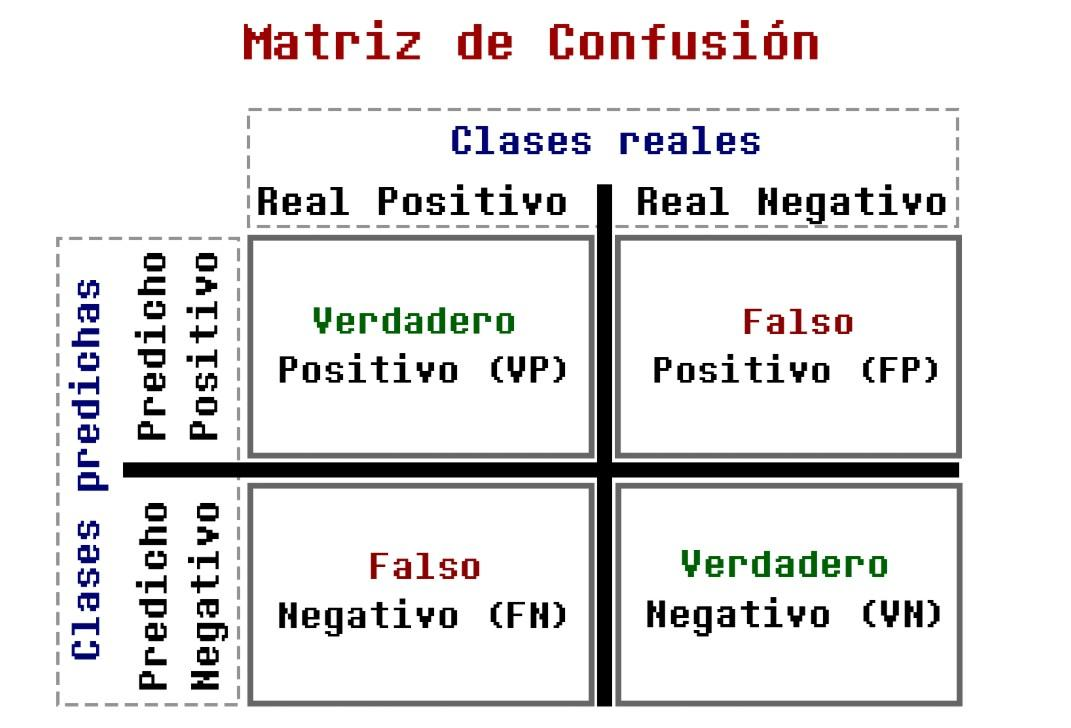
\includegraphics[width=0.8\textwidth]{images/fig21.jpg}
		\caption{ Matriz de Confusión .  \cite{dialektico_metricas}.}
		\label{fig:MatrizConf}
	\end{figure}
	
	
	\subsubsection{Estrategia de ajuste fino (\textit{Fine-Tuning})}
	
	El \textit{Transfer Learning} es una estrategia ampliamente empleada en visión por computadora que consiste en reutilizar el conocimiento adquirido por un modelo previamente entrenado en un dominio amplio —por ejemplo, ImageNet— para resolver una tarea diferente con un conjunto de datos más reducido. En lugar de entrenar una CNN desde cero, esta técnica permite aprovechar representaciones visuales generales aprendidas en el entrenamiento original, como bordes, texturas, contornos u objetos básicos, las cuales son útiles en una amplia variedad de problemas de clasificación o reconocimiento \cite{pan2010}.
	
	Diversos estudios han demostrado que las representaciones aprendidas en las primeras capas de una red neuronal son altamente transferibles, mientras que las capas profundas tienden a ser más específicas del dominio original \cite{yosinski2014}. Esta propiedad permite reutilizar eficazmente los niveles bajos de la red, reduciendo la necesidad de grandes volúmenes de datos en la tarea objetivo.
	
	Dentro del marco del \textit{Transfer Learning} existen diversas estrategias para reutilizar modelos preentrenados, entre las que destacan: el uso de la red como extractor de características, la sustitución de la capa de clasificación final, y el ajuste parcial o completo de los pesos del modelo. Entre estas, la técnica más flexible es el \textit{Fine-Tuning}, la cual consiste en ajustar selectivamente los parámetros del modelo para adaptarlo al nuevo dominio \cite{oquab2014}. De este modo, mientras que el \textit{Transfer Learning} describe el concepto general de reutilización de conocimiento, el \textit{Fine-Tuning} representa una estrategia específica orientada a refinar las representaciones internas del modelo.
	
	Desde el punto de vista operativo, el \textit{Fine-Tuning} implica decidir qué capas de la red se mantienen congeladas y cuáles se actualizan en el proceso del entrenamiento. Las capas congeladas conservan sus pesos originales, preservando patrones generales previamente aprendidos y reduciendo el riesgo de sobreajuste, especialmente cuando el conjunto de datos objetivo es limitado \cite{howard2018}. Por otro lado, la descongelación parcial permite que las capas más profundas adapten sus representaciones a características específicas del nuevo dominio, incrementando la capacidad de especialización del modelo \cite{yosinski2014}.
	
	No obstante, el \textit{Fine-Tuning} también presenta riesgos teóricos, siendo el más relevante el \textit{catastrophic forgetting}, fenómeno mediante el cual el modelo pierde o sobrescribe el conocimiento previamente adquirido al adaptarse a una nueva tarea \cite{french1999}. Este problema puede surgir cuando los ajustes en los parámetros son demasiado agresivos, alterando representaciones previamente estables. Para mitigar este efecto, se recomienda emplear tasas de aprendizaje reducidas, aplicar estrategias de descongelación progresiva y utilizar técnicas de regularización que limiten cambios abruptos en los pesos \cite{howard2018}.
	
	El \textit{Fine-Tuning} requiere la toma de decisiones técnicas que influyen directamente en la estabilidad del entrenamiento y en la efectividad de la transferencia de conocimiento. Entre estas decisiones destacan la selección de las capas a ajustar, la profundidad del \textit{fine-tuning}, la tasa de aprendizaje empleada y el número de épocas de entrenamiento, las cuales deben ser cuidadosamente configuradas para lograr una adaptación adecuada sin incurrir en sobreajuste \cite{yosinski2014}.
	
	En la mayoría de las CNN preentrenadas, las capas se organizan jerárquicamente de la siguiente manera \cite{yosinski2014}:
	\begin{itemize}
		\item \textbf{Capas bajas (\textit{early layers}):} capturan bordes, texturas y gradientes.
		\item \textbf{Capas medias (\textit{mid-level layers}):} representan patrones compuestos, contornos y partes de objetos.
		\item \textbf{Capas profundas (\textit{high-level layers}):} codifican características semánticas específicas del dominio original.
	\end{itemize}
	
	En arquitecturas como VGG, ResNet o EfficientNet, una estrategia común consiste en congelar entre el 30\% y el 60\% de las capas iniciales, y permitir que las últimas dos a cuatro etapas convolucionales se actualicen. Este enfoque ofrece un equilibrio adecuado entre estabilidad del conocimiento previo y capacidad de adaptación al nuevo dominio.
	
	La cantidad de capas descongeladas puede variar en función del tamaño y la complejidad del conjunto de datos objetivo. En escenarios con pocos datos, es recomendable aplicar un \textit{fine-tuning} superficial, donde únicamente se descongela el último bloque convolucional. Esto reduce el riesgo de \textit{catastrophic forgetting} y limita la desviación del modelo respecto a las representaciones previamente aprendidas. Por el contrario, cuando el conjunto de datos es más amplio o difiere significativamente del dominio original, se prefiere un \textit{fine-tuning} profundo, en el cual se actualizan múltiples bloques de la red. Estudios empíricos sugieren que descongelar entre el 20\% y el 40\% de las capas puede ofrecer un equilibrio adecuado entre especialización y estabilidad \cite{yosinski2014}.
	
	La tasa de aprendizaje empleada en el \textit{fine-tuning} es uno de los factores más críticos del proceso. Dado que el modelo parte de parámetros previamente optimizados, actualizaciones excesivas pueden deteriorar las representaciones útiles ya aprendidas. Por esta razón, las capas preentrenadas suelen ajustarse con tasas de aprendizaje en el rango de $10^{-4}$ a $10^{-5}$, mientras que las capas añadidas (entrenadas desde cero) pueden utilizar valores ligeramente mayores, típicamente entre $10^{-3}$ y $10^{-4}$. Tasas de aprendizaje elevadas provocan cambios abruptos en los pesos, mientras que valores más bajos permiten una adaptación más estable, aunque a costa de una convergencia más lenta \cite{howard2018}.
	
	En cuanto al número de épocas, el \textit{fine-tuning} suele requerir menos iteraciones que el entrenamiento desde cero. Para conjuntos de datos pequeños, entre 5 y 20 épocas suelen ser suficientes, mientras que para tareas más complejas o con mayor divergencia respecto al dominio original pueden requerirse entre 15 y 50 épocas. En escenarios donde se descongelan múltiples capas profundas, el entrenamiento puede extenderse hasta 100 épocas. No obstante, es habitual emplear técnicas como \textit{early stopping} para prevenir el sobreajuste, ya que el modelo puede memorizar rápidamente los datos cuando se ajustan demasiados parámetros \cite{pan2010}.
	
	Para mejorar la estabilidad del \textit{fine-tuning}, se incorporan diversas técnicas de regularización, tales como \textit{weight decay} en rangos de $10^{-4}$ a $10^{-5}$, el uso de \textit{dropout} en capas densas \cite{oquab2014}, el incremento del \textit{data augmentation} y, en particular, la estrategia de \textit{gradual unfreezing}, en donde las capas se descongelan de manera progresiva a lo largo del entrenamiento. Este enfoque permite una adaptación más controlada y reduce el riesgo de pérdida del conocimiento previamente adquirido \cite{howard2018}.
	
	La decisión sobre cuántas capas descongelar depende en gran medida del tamaño del conjunto de datos y de su similitud semántica con el dominio de preentrenamiento. La siguiente tabla resume las recomendaciones más comunes reportadas en la literatura.
	
	
	\rowcolors{2}{rowblue}{white}
	
	\small
	\renewcommand{\arraystretch}{1.2}
	
	\begin{longtable}{|p{4.5cm}|p{8.0cm}|}
		\caption{Profundidad recomendada del \textit{fine-tuning} según el tamaño del dataset objetivo} \\
		\hline
		\rowcolor{headerblue}
		\headercell{Tamaño del dataset nuevo} &
		\headercell{Estrategia recomendada} \\
		\hline
		\endfirsthead
		
		\hline
		\rowcolor{headerblue}
		\headercell{Tamaño del dataset nuevo} &
		\headercell{Estrategia recomendada} \\
		\hline
		\endhead
		
		\rowcolors{1}{rowblue}{white}
		
		Muy pequeño ($< 2k$ imágenes) &
		Congelar la mayoría de las capas; aplicar \textit{fine-tuning} superficial sobre el último bloque \\
		\hline
		
		Medio ($2k$--$20k$ imágenes) &
		Descongelar los últimos bloques convolucionales y utilizar una tasa de aprendizaje baja \\
		\hline
		
		Grande ($> 20k$ imágenes) &
		Aplicar \textit{fine-tuning} profundo, combinado con técnicas de regularización \\
		\hline
		
		Muy diferente al dominio original &
		Descongelar múltiples bloques para permitir una adaptación significativa del modelo \\
		\hline
		
	\end{longtable}
	
	\rowcolors{2}{rowblue}{white}
	
	\small
	\renewcommand{\arraystretch}{1.2}
	
	\begin{longtable}{|p{3.2cm}|p{3.5cm}|p{3.5cm}|p{3.5cm}|}
		\caption{Parámetros comunes del \textit{Fine-Tuning}, su función y recomendaciones de uso \cite{yosinski2014, pan2010, oquab2014, howard2018, srivastava2014}} \\
		\hline
		\rowcolor{headerblue}
		\headercell{Parámetro del Fine-Tuning} &
		\headercell{¿Para qué sirve?} &
		\headercell{Cuándo usarlo} &
		\headercell{Cuándo NO usarlo} \\
		\hline
		\endfirsthead
		
		\hline
		\rowcolor{headerblue}
		\headercell{Parámetro del Fine-Tuning} &
		\headercell{¿Para qué sirve?} &
		\headercell{Cuándo usarlo} &
		\headercell{Cuándo NO usarlo} \\
		\hline
		\endhead
		
		\rowcolors{1}{rowblue}{white}
		
		Congelación de capas iniciales &
		Preserva filtros universales (bordes, texturas simples) previamente aprendidos &
		Cuando el dataset es pequeño o similar al dominio original &
		Cuando el dominio es muy distinto o se requieren nuevas representaciones visuales \\
		\hline
		
		Descongelación de capas profundas &
		Permite adaptar representaciones especializadas al nuevo dominio &
		Cuando el dataset es grande o semánticamente diferente &
		En datasets pequeños, ya que puede provocar sobreajuste y \textit{forgetting} \\
		\hline
		
		Descongelación progresiva (\textit{gradual unfreezing}) &
		Reduce el \textit{catastrophic forgetting} mediante actualización escalonada &
		Cuando se requiere un ajuste profundo pero estable &
		Cuando se prioriza rapidez o el dominio es muy similar \\
		\hline
		
		Tasa de aprendizaje baja ($10^{-4}$--$10^{-5}$) &
		Evita sobrescribir representaciones útiles del preentrenamiento &
		Para ajustar capas preentrenadas o dominios sensibles &
		Cuando se entrena únicamente la nueva capa de clasificación \\
		\hline
		
		Tasa de aprendizaje moderada ($10^{-3}$--$10^{-4}$) &
		Acelera la adaptación del clasificador añadido &
		Al entrenar capas nuevas desde cero (\textit{head}) &
		En capas profundas preentrenadas (puede degradar el conocimiento previo) \\
		\hline
		
		Número de épocas reducido (5--20) &
		Evita sobreajuste rápido en datasets pequeños &
		Cuando se ajustan pocas capas o hay pocos datos &
		En tareas complejas donde se requiere adaptación profunda \\
		\hline
		
		Número de épocas alto (30--100) &
		Permite reentrenar múltiples bloques en tareas complejas &
		Cuando el dominio difiere significativamente del original &
		En datasets pequeños (provoca sobreajuste) \\
		\hline
		
		\textit{Weight decay} ($10^{-4}$--$10^{-5}$) &
		Controla el sobreajuste limitando la magnitud de los pesos &
		En \textit{fine-tuning} profundo o datasets medianos/grandes &
		En \textit{fine-tuning} superficial con pocos parámetros ajustables \\
		\hline
		
		\textit{Dropout} adicional &
		Reduce el sobreajuste en capas densas &
		Cuando se entrena un clasificador nuevo o dataset pequeño/medio &
		En arquitecturas sin capas densas adicionales \\
		\hline
		
		Aumentación de datos agresiva &
		Mejora la generalización y reduce el \textit{forgetting} &
		En datasets pequeños o con alta variabilidad &
		Cuando las transformaciones alteran la semántica de la tarea \\
		\hline
		
	\end{longtable}
	El \textit{Fine-Tuning} es un procedimiento relevante dentro del \textit{Transfer Learning} que permite adaptar modelos previamente entrenados a nuevos contextos mediante el aprovechamiento de sus representaciones internas. Su combinación de estabilidad, eficiencia computacional y capacidad de generalización lo ha convertido en una estrategia ampliamente utilizada en tareas de visión por computadora.
	
	\subsubsection{Aumentación de datos (\textit{Data Augmentation})}
	
	La aumentación de datos es una de las estrategias fundamentales para mejorar la capacidad de generalización en tareas de visión por computadora, especialmente cuando los conjuntos de datos son limitados o presentan baja variabilidad. Su objetivo principal es incrementar la diversidad estadística del conjunto de entrenamiento mediante la generación de nuevas muestras sintéticas a partir de transformaciones aplicadas a las imágenes originales, sin necesidad de recolectar datos adicionales. Desde una perspectiva teórica, este proceso permite que el modelo aprenda representaciones más robustas y menos sensibles a variaciones irrelevantes en la apariencia de los objetos, favoreciendo la invariancia ante factores comunes en escenarios reales, como cambios de iluminación, perspectiva, posición o ruido \cite{shorten2019, perez2017}.
	
	Las técnicas de aumentación pueden agruparse en dos grandes categorías: aumentación geométrica y aumentación fotométrica. La aumentación geométrica modifica la estructura espacial de la imagen mediante operaciones como rotaciones, traslaciones, escalado, volteos horizontales o recortes aleatorios. Estas transformaciones obligan al modelo a aprender características invariantes a cambios de posición y forma. Por otro lado, la aumentación fotométrica actúa sobre las propiedades de color y luminancia, incorporando variaciones en brillo, contraste, saturación, gamma o la adición de ruido, lo que permite mejorar la robustez frente a condiciones ambientales y variaciones entre dispositivos de captura \cite{shorten2019, yang2022}.
	
	Diversos estudios han demostrado que la combinación adecuada de ambas categorías puede generar mejoras significativas en métricas de desempeño como la exactitud, la medida F1 y la capacidad de generalización del modelo, particularmente en escenarios donde el conjunto de entrenamiento es reducido y propenso al sobreajuste. En este sentido, transformaciones como recortes, rotaciones moderadas y volteos controlados han mostrado ser efectivas para incrementar la diversidad de los datos sin comprometer su coherencia semántica \cite{perez2017}.
	
	La aplicación de aumentación de datos debe realizarse con precaución, ya que ciertas transformaciones pueden alterar la semántica de la clase. En tareas que dependen de la orientación espacial, como el reconocimiento de señas estáticas en Lengua de Señas Mexicana (LSM), transformaciones excesivas —como rotaciones pronunciadas, recortes agresivos o volteos inadecuados— pueden modificar el significado de la seña, introduciendo ruido contradictorio en el entrenamiento. Estudios recientes en reconocimiento de gestos han demostrado que no todas las transformaciones aportan beneficios, y que su efectividad depende directamente de la naturaleza del problema y del diseño del conjunto de datos \cite{yang2022}. Debido a que un esquema de aumentación demasiado agresivo puede generar distribuciones artificiales alejadas del dominio real, provocando una generalización deficiente y un comportamiento inestable del modelo en escenarios de aplicación \cite{yang2022}.
	
	\begin{figure}[H]
		\centering
		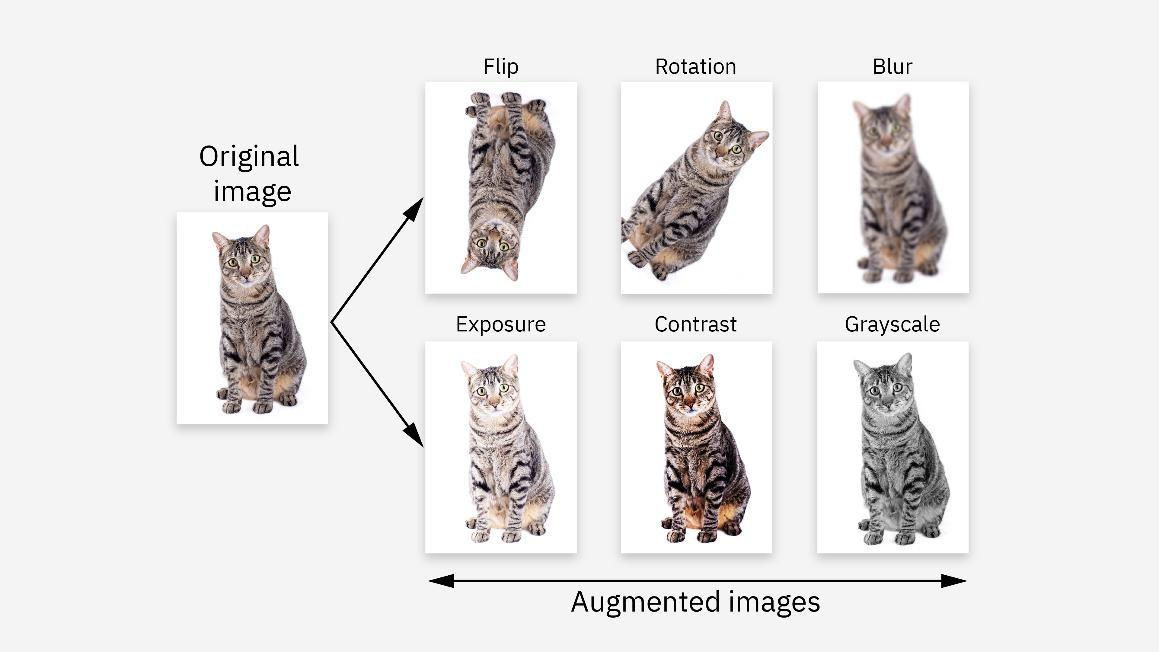
\includegraphics[width=0.8\textwidth]{images/fig22.jpg}
		\caption{ Aplicacion de Data Augmentation  .  \cite{ibm_data_augmentation}.}
		\label{fig:MatrizConf}
	\end{figure}
	
	Por estas razones la selección de transformaciones debe estar alineada con la naturaleza del problema, el comportamiento esperado del modelo y la estructura del conjunto de datos. En aplicaciones de reconocimiento de señas, por ejemplo, los ajustes leves de brillo, variaciones controladas de contraste y recortes moderados pueden enriquecer la variabilidad sin afectar la identidad de la seña, mientras que las transformaciones que alteran la forma global de la mano, su orientación original o la posición crítica de los dedos deben restringirse o evitarse. Un proceso de aumentación bien diseñado contribuye directamente a un modelo más robusto, capaz de generalizar adecuadamente ante escenarios reales y condiciones de captura no controladas. 
	\subsection{Representación de gestos basada en landmarks y extracción de características}
	El reconocimiento de gestos en visión por computadora ha experimentado una evolución significativa en los últimos años, pasando de enfoques basados en el procesamiento directo de imágenes a métodos que utilizan representaciones estructuradas del objeto de interés. Dentro de estas representaciones, los \textit{landmarks} se han consolidado como una alternativa eficiente para modelar la geometría de elementos complejos como la mano humana.
	
	Un landmark se define como un punto clave que describe una posición relevante dentro de una estructura, generalmente asociada a características geométricas o articulares. Estos puntos permiten abstraer la información visual en un conjunto reducido de coordenadas, lo que disminuye considerablemente la dimensionalidad del problema en comparación con el uso de imágenes completas \cite{bishop2006pattern}.
	
	Este tipo de representación funciona en aplicaciones donde se requiere procesamiento en continuo o donde los recursos computacionales son limitados, como en dispositivos móviles. Al trabajar con vectores de características en lugar de matrices de píxeles, se facilita la implementación de modelos de aprendizaje automático más ligeros y eficientes \cite{geron2019hands}.
	
	Uno de los frameworks más utilizados para la detección de landmarks en tiempo real es MediaPipe, desarrollado por Google como una solución para la construcción de pipelines de percepción eficientes \cite{lugaresi2019mediapipe}. Dentro de este framework, el módulo \textit{MediaPipe Hands} permite la detección y seguimiento de manos mediante el uso de modelos optimizados para ejecución en dispositivos con recursos limitados \cite{mediapipe_hands}.
	
	MediaPipe Hands emplea una arquitectura de dos etapas: en la primera se detecta la región de interés correspondiente a la mano dentro de la imagen, y en la segunda se realiza la estimación precisa de los puntos clave. Como resultado, el sistema es capaz de identificar hasta 21 landmarks por cada mano, los cuales representan articulaciones y puntos relevantes como la muñeca, nudillos y puntas de los dedos \cite{zhang2020mediapipehands}.
	
	Estos puntos permiten modelar la estructura de la mano de forma consistente, proporcionando una base sólida para tareas de clasificación de gestos. Además, al tratarse de un sistema optimizado para ejecución continua, su integración en aplicaciones móviles es viable sin necesidad de hardware especializado de alto rendimiento.
	
	Cada uno de los landmarks detectados por MediaPipe Hands se representa mediante un conjunto de coordenadas tridimensionales normalizadas (x, y, z). Las componentes x e y corresponden a la posición relativa del punto dentro de la imagen, mientras que la componente z proporciona una estimación de la profundidad respecto a la cámara \cite{mediapipe_hands}.
	
	Desde el punto de vista de la visión por computadora, estas coordenadas forman parte de un sistema de referencia que permite describir la posición de los puntos dentro de un espacio bidimensional o tridimensional \cite{szeliski2010computer}. A partir de estos valores, es posible construir un vector de características que represente la configuración completa de la mano.
	
	Por ejemplo, considerando 21 landmarks y únicamente las coordenadas (x, y), se obtiene un vector de 42 dimensiones. Si se incluye la componente z, el vector se extiende a 63 dimensiones. Esta representación compacta es significativamente más eficiente que el uso de imágenes completas, las cuales pueden contener miles o millones de valores.
	
	\subsubsection{Transformación a coordenadas relativas}
	
	Uno de los principales desafíos es la variabilidad espacial de la mano dentro de la imagen. Factores como la posición, orientación y distancia respecto a la cámara pueden afectar directamente los valores absolutos de las coordenadas detectadas, introduciendo variaciones no deseadas en la representación de los datos.
	
	Para mitigar este problema, se emplea una transformación hacia coordenadas relativas, la cual consiste en redefinir el sistema de referencia tomando como origen un punto específico de la mano, comúnmente la muñeca (landmark 0 en MediaPipe Hands). Este enfoque permite que la representación sea invariante a traslaciones dentro del plano de la imagen.
	
	Sea un conjunto de landmarks definido como:
	
	\[
	L = \{(x_i, y_i, z_i)\}_{i=1}^{N}
	\]
	
	donde \( N = 21 \) corresponde al número de puntos detectados. La transformación a coordenadas relativas se define como:
	
	\[
	x_i' = x_i - x_{ref}, \quad y_i' = y_i - y_{ref}, \quad z_i' = z_i - z_{ref}
	\]
	
	donde \((x_{ref}, y_{ref}, z_{ref})\) corresponde al landmark de referencia.
	
	Este procedimiento traslada la nube de puntos al origen del sistema de coordenadas, eliminando la dependencia de la posición absoluta de la mano dentro de la imagen. Desde el punto de vista geométrico, esta operación corresponde a una transformación de traslación en el espacio euclidiano \cite{szeliski2010computer}.
	
	El uso de coordenadas relativas permite capturar únicamente la configuración estructural de la mano, es decir, las relaciones espaciales entre los dedos y articulaciones, lo cual es fundamental para tareas de clasificación de gestos.
	
	
	Aun cuando la transformación a coordenadas relativas elimina la dependencia de la posición absoluta, persisten variaciones asociadas a la escala y al encuadre de la mano dentro de la imagen. Estas variaciones pueden afectar la consistencia del vector de características y, en consecuencia, el desempeño del modelo de clasificación.
	
	Para reducir este efecto, se emplea un proceso de normalización de las coordenadas basado en el ajuste de los valores mínimos dentro del conjunto de puntos. Este procedimiento consiste en trasladar todos los puntos de tal forma que el valor mínimo de cada eje corresponda al origen.
	
	Sea el conjunto de coordenadas relativas definido como:
	
	\[
	L' = \{(x_i', y_i')\}_{i=1}^{N}
	\]
	
	Se definen los valores mínimos como:
	
	\[
	x_{min} = \min_{i}(x_i'), \quad y_{min} = \min_{i}(y_i')
	\]
	
	La normalización se realiza mediante:
	
	\[
	x_i'' = x_i' - x_{min}, \quad y_i'' = y_i' - y_{min}
	\]
	
	Este proceso garantiza que todos los valores del vector de características sean no negativos y se encuentren en un rango consistente, reduciendo la variabilidad asociada a cambios en la posición y tamaño de la mano dentro del campo visual.
	
	La normalización de los datos es una etapa fundamental en el preprocesamiento, ya que mejora la estabilidad numérica y facilita la convergencia de los modelos en el entrenamiento \cite{bishop2006pattern}.
	
	Ya obtenidas las coordenadas normalizadas, se procede a la construcción del vector de características que será utilizado como entrada para el modelo de clasificación.
	
	Dado un conjunto de \( N = 21 \) landmarks y considerando únicamente las coordenadas bidimensionales, el vector de características se define como la concatenación de todos los puntos:
	
	\[
	\mathbf{f} = [x_1'', y_1'', x_2'', y_2'', \dots, x_N'', y_N'']
	\]
	
	lo que da lugar a un vector de dimensión \( 2N = 42 \). En caso de incluir la componente de profundidad, el vector se extiende a:
	
	\[
	\mathbf{f} = [x_1'', y_1'', z_1'', \dots, x_N'', y_N'', z_N'']
	\]
	
	con dimensión \( 3N = 63 \).
	
	Esta representación transforma la información espacial de la mano en un vector numérico estructurado, adecuado para su procesamiento mediante algoritmos de aprendizaje automático. A diferencia de las representaciones basadas en imágenes, esta aproximación reduce significativamente la dimensionalidad del problema, permitiendo el uso de modelos más simples y eficientes \cite{geron2019hands}.
	
	Además, al conservar las relaciones espaciales entre los puntos, el vector de características mantiene la información necesaria para distinguir entre diferentes configuraciones gestuales.
	
	\begin{figure}[H]
		\centering
		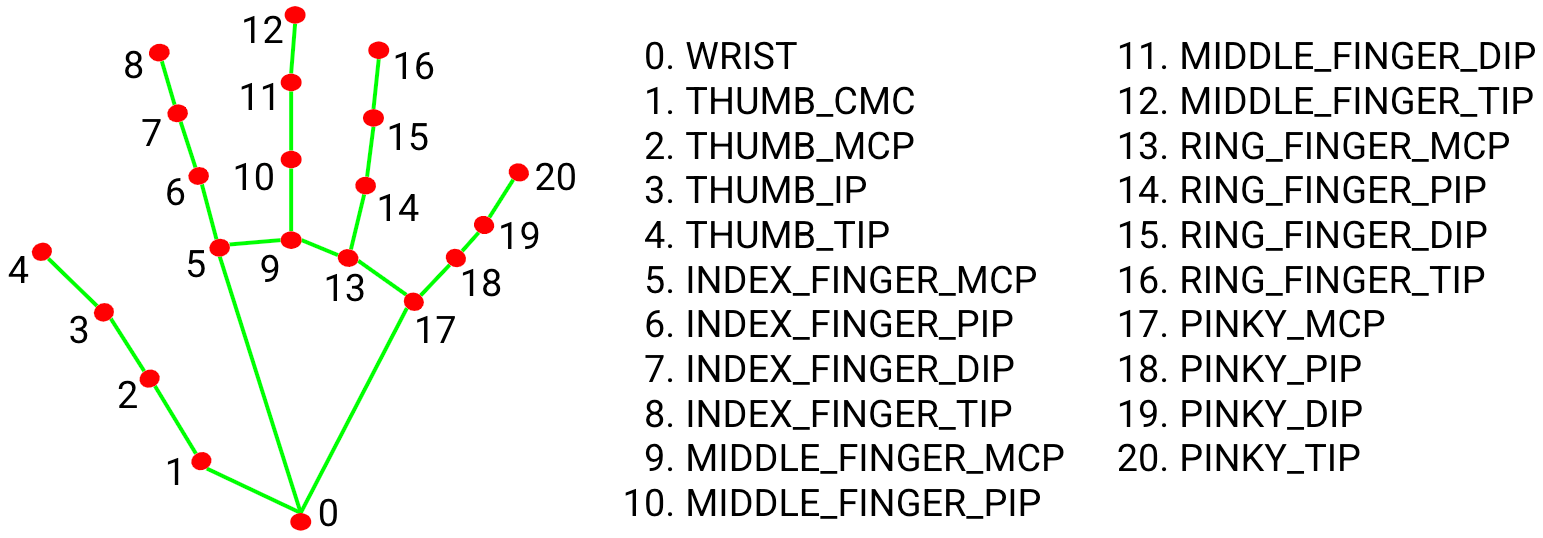
\includegraphics[width=0.7\textwidth]{images/fig23.png}
		\caption{Representación de los 21 landmarks detectados en una mano mediante MediaPipe Hands.\cite{mediapipe_hands}}
		\label{fig:landmarks}
	\end{figure}
	
	El reconocimiento de gestos basado en landmarks requiere el uso de modelos de clasificación capaces de identificar patrones dentro de vectores de características. Estos modelos reciben como entrada una representación numérica estructurada y generan como salida una etiqueta correspondiente a una clase determinada.
	
	Dentro del aprendizaje automático supervisado, existen diversos algoritmos utilizados para tareas de clasificación, tales como máquinas de soporte vectorial (SVM), árboles de decisión, bosques aleatorios y redes neuronales artificiales. Estos modelos buscan aprender una función que permita separar las distintas clases dentro del espacio de características \cite{bishop2006pattern}.
	
	La elección del modelo depende de factores como la dimensionalidad de los datos, la complejidad del problema y los recursos computacionales disponibles. En el caso de representaciones basadas en landmarks, donde los datos se presentan como vectores numéricos de baja o media dimensionalidad, es posible emplear modelos eficientes que capturen relaciones espaciales entre los puntos.
	
	
	\subsubsection{Implementación e inferencia de modelos de aprendizaje automático en dispositivos móviles}

	Android es un sistema operativo móvil basado en el kernel de Linux y desarrollado por Google como parte del Android Open Source Project (AOSP). Su arquitectura se organiza en múltiples capas, entre las que destacan el Android Runtime (ART), las bibliotecas nativas, el Application Framework y un conjunto de interfaces de programación de aplicaciones (APIs) que permiten la interacción con el hardware del dispositivo \cite{android_architecture}. Esta estructura modular ha permitido que Android evolucione hacia un ecosistema robusto, flexible y compatible con una amplia variedad de dispositivos con diferentes capacidades de cómputo.
	
	En los últimos años, el incremento en la capacidad de procesamiento de los dispositivos móviles, junto con la incorporación de hardware especializado como unidades de procesamiento gráfico (GPU), procesadores digitales de señal (DSP) y unidades de procesamiento neuronal (NPU), ha impulsado el desarrollo del paradigma conocido como \textit{machine learning on-device}. Este enfoque consiste en ejecutar modelos de aprendizaje automático directamente en el dispositivo, sin necesidad de depender de servicios en la nube, lo que permite reducir la latencia, mejorar la privacidad de los datos y garantizar el funcionamiento en entornos con conectividad limitada \cite{wu2019machine}.
	
	La implementación de modelos de aprendizaje automático en dispositivos móviles se centra principalmente en la etapa de inferencia, es decir, en la utilización de modelos previamente entrenados para realizar predicciones a partir de nuevos datos de entrada. A diferencia del entrenamiento, que requiere grandes volúmenes de datos y recursos computacionales elevados, la inferencia puede ejecutarse de manera eficiente en dispositivos móviles siempre que los modelos sean adecuadamente optimizados.
	
	Para facilitar este proceso, se han desarrollado frameworks especializados como TensorFlow Lite, una biblioteca diseñada para ejecutar modelos de aprendizaje automático en entornos con recursos limitados. TensorFlow Lite permite optimizar modelos mediante técnicas como la cuantización y la reducción de precisión numérica, lo que disminuye el uso de memoria y mejora los tiempos de respuesta en la clasificación \cite{tensorflow_lite}. Estas características son fundamentales para aplicaciones que requieren procesamiento en tiempo real.
	
	Sin embargo, no todos los modelos de aprendizaje automático presentan el mismo nivel de compatibilidad con entornos móviles. Algoritmos tradicionales como las máquinas de soporte vectorial (SVM), los bosques aleatorios (Random Forest) o los métodos basados en vecinos más cercanos (KNN) no cuentan con una integración nativa dentro de frameworks de inferencia móvil como TensorFlow Lite. Aunque existen alternativas para implementar este tipo de modelos mediante soluciones personalizadas, dichas aproximaciones suelen requerir procesos adicionales de adaptación y pueden presentar limitaciones en términos de optimización, portabilidad y eficiencia computacional dentro de dispositivos con recursos limitados.
	
	Ademas, las redes neuronales artificiales, incluyendo arquitecturas como el perceptrón multicapa (MLP) y otras variantes de aprendizaje profundo, poseen una integración directa con frameworks modernos de inferencia móvil. Esto permite convertir y desplegar modelos de manera eficiente en dispositivos Android utilizando herramientas como TensorFlow Lite, facilitando la ejecución local del proceso de clasificación y aprovechando, cuando el hardware lo permite, aceleradores especializados como GPU o NPU para mejorar el rendimiento y reducir el consumo energético.
	
	Frameworks como MediaPipe permiten la construcción de pipelines de percepción que integran procesos de captura, procesamiento y extracción de características directamente en el dispositivo \cite{lugaresi2019mediapipe}. En particular, el uso de representaciones basadas en landmarks reduce significativamente la cantidad de datos que deben ser procesados por los modelos de clasificación, favoreciendo la eficiencia del sistema.
	
	En el reconocimiento de gestos, la combinación de técnicas de extracción de características basadas en landmarks con modelos de clasificación ligeros permite desarrollar sistemas capaces de operar completamente en el dispositivo móvil.
	
	% ==================================================
